\documentclass[11pt,a4paper,margin=1.5in]{article}
\usepackage{amsfonts}
\usepackage{amssymb}
\usepackage{amsmath}
\usepackage{color}
\usepackage{setspace}
\usepackage{dcolumn}
\newcolumntype{d}[1]{D{.}{.}{#1}}
\usepackage{multicol}

\usepackage[dvipsnames]{xcolor}
\definecolor{cobalt}{rgb}{0.0, 0.28, 0.67}
\definecolor{darkblue}{rgb}{0.0, 0.0, 0.55}
\definecolor{darkpowderblue}{rgb}{0.0, 0.2, 0.6}
\definecolor{egyptianblue}{rgb}{0.06, 0.2, 0.65}
\usepackage[pdfencoding=auto]{hyperref}
\hypersetup{
    colorlinks=true,
    linkcolor=black,%egyptianblue,
    citecolor=black,%blue,
    filecolor=magenta,      
    urlcolor=darkblue,
}
\hypersetup{pdfstartview={XYZ null null 0.80}}

\usepackage[FIGTOPCAP]{subfigure}
\usepackage{IEEEtrantools}
\usepackage{extsizes}
\usepackage{tikz}
\usepackage{pgfplots}
%\usepackage{subcaption}
\usepackage{booktabs}
\usepackage[flushleft]{ threeparttable}
\usepackage{graphicx}
\usepackage{epstopdf}
\usepackage{parskip}
\usepackage{geometry}
\usepackage{pdflscape}
\usepackage{rotating}
%\usepackage{afterpage}
\usepackage{multirow}
\usepackage{natbib}
\usepackage{xfrac}
\usepackage{paralist}
\usepackage{fancyhdr}
%\usepackage[nomarkers, nolists]{endfloat}
%\renewcommand{\efloatseparator}{\vspace{3in}}

%\theoremstyle{plain}
\newtheorem{assumption}{Assumption}

\setlength{\parindent}{12pt}
%\onehalfspacing
\doublespacing

\defcitealias{IMF:2013}{IMF, 2013}
\defcitealias{Blanchard:2016}{Blanchard, 2016}

\title{Fiscal Monetary Services and Inflation}
%\thanks{
%	I'd like to thank Bill Barnett, David Beckworth, Markus Brunnermeier, Josh Hendrickson, Tom Holden, John Nana Francois, Peter Ireland, Eric Leeper, Ryan Mattson, and Ricardo Nunes for their helpful comments and advice on this and previous versions of this paper.
%	I'd also like to thank the numerous seminar participants at the University of Kansas, Utah State University, Southern Utah University, and various conferences for their invaluable feedback.}}
\author{Andrew Keinsley\thanks{Associate Professor of Economics, Weber State University --- Email: andrewkeinsley@weber.edu -- Address: Department of Economics WB 226, 1337 Edvalson St, Ogden, UT 84408-3807 } \\  {\small Weber State University}}
%\date{ {\bf Preliminary: Comments Welcome}  \\ This Version: \today}

\begin{document}
\maketitle
\thispagestyle{empty}

\begin{abstract}
\noindent In this paper I use a Fisher ideal index to track the monetary services provided by marketable US government debt.
To do so, I first develop the theory necessary to consider using such a statistical index number, show how the value of these fiscal monetary services expand the fiscal capacity to borrow, and provide evidence that the monetary services are primarily safety services.
I then use \citet{Jorda:2005} projections to estimate the impact of such monetary services on inflation.
I find that a one-percent increase in fiscal monetary services produces a positive and statistically-significant inflationary response that peaks between four and five basis points and persists for ten months. 
Given that the average growth rate of the fiscal monetary services in my sample is 2.5 percent, the impact is also economically significant.
Together, these results suggest that there is a fiscal channel of inflation through the monetary services Treasury debt provides, though a small-scale New Keynesian model implies that it is not through the standard channels predicted by the fiscal theory of the price level.

%monetary services channel to the fiscal theory of the price level.
\end{abstract}
\vspace{2em}

\noindent{Keywords}: Fiscal Theory of the Price Level, Aggregation Theory, Inflation, Fiscal Debt
\newpage
\setcounter{page}{1}


\section{Introduction}

% Introduce the Topic and its Imporance
The fiscal response to the COVID crisis in the US and the ensuing rise of inflation and interest rates has brought the concept of ``fiscal capacity" back into the spotlight. 
Despite growing debt levels, borrowing costs trended downward from the 1980s until the US financial crisis in the late 2000s.
%Forecasters, despite accelerating debt levels, suggest that short-term interest rates will peak somewhere around two percent in the post-COVID cycle. 
All of this suggests that there must be more to the fiscal-capacity discussion than just the stock of outstanding principal values.
If that additional component could be discovered, could it also shed light on the connection between debt and the macroeconomy, like the fiscal theory of the price level (FTPL)?

% Brief Literature Review
\citet{Krishnamurthy-VissingJorgensen:2012}, \citet{Krishnamurthy-VissingJorgensen:2013}, and \citet{Nagel:2016}---to name just a few---have established that the value of fiscal debt in the US is much more than the sum of its outstanding stock of principal. 
\citet*{Caballero-Farhi-Gourinchas:2017} build on this idea to explain historically low borrowing costs in the face of historically high debt levels.
More recently, \citet*{Brunnermeier-Merkel-Sannikov:2022} applied these concepts to the fiscal capacity and the FTPL literatures. 
They show that the demand side of this debt market raises the borrowing limits of the fiscal authority because the additional debt provides safety or transaction services, which I'll refer to more generally as monetary services.\footnote{
	These monetary services generally include the aforementioned transactions services as well as other attributes such as liquidity, safety, use as collateral, etc.}
Theoretically, they show that the inclusion of these monetary services disrupt the traditional FTPL channel \citep[see][as a seminal example]{Leeper:1991} and, along with the empirical results of \citet{Jiang-etal:2019}, suggest that this channel is important in the valuation of Treasury debt. 
%, but introduce the possibility of other channels.\footnote{
%	\citet{Cui-Soren:2019} find that the bubble term in their model with low interest rates is primarily composed of liquidity services as well.}
This paper explores this monetary service channel in more depth, aiding in our understanding of debt dynamics and their impact on the economy as a whole. 

% Purpose of this paper...
The purpose and contribution of this paper is two-fold.
%to measure the monetary services of marketable fiscal debt in the US and to estimate their impact on inflation.
% Contribution to the literature
%The contribution of this paper is two-fold.
First, I measure the monetary services established as theoretically important in the literature.
This measure provides additional insight not only into how debt and its dynamics impact the greater economy, but also how global events impact the monetary services of outstanding fiscal debt.
If fiscal monetary services do provide additional fiscal capacity and influence inflation dynamics as \citet{Brunnermeier-Merkel-Sannikov:2022} theorize, then understanding the extent of the impact is vital to policy makers. 
Second, I provide both theoretical and empirical evidence of a fiscal inflation channel through the rate premiums (liquidity and/or safety) created by those monetary services.
That is, while the inflation is derived from an externality of fiscal policy, it is not though the standard channels predicted by the FTPL. 
%via these monetary services, though I also show that this result is through the liquidity premiums in the model, not the standard channels predicted by the FTPL.
%monetary services channel to the fiscal theory of the price level.
%The debate between the monetarist view of inflation and those behind the FTPL has been long and arduous.
Showing that fiscal debt influences inflation through its monetary properties suggests that these two theories may not be as different as suspected and provides a potential bridge between the two.
Together, the results within this paper provide a contribution to the monetary aggregation, fiscal capacity, and inflation literatures.

% Results 1
The first result of this paper is the derivation of the underlying theory for the quantity index of interest.
As is noted in the extensive monetary aggregation literature \citep[e.g.][]{Barnett:1978, Barnett:1980, Barnett-Serletis:2000}, a statistical index used to track a true aggregate like the one considered here must be derived from an optimizing agent.
Therefore, I consider a partial equilibrium model of the representative household which incorporates the monetary services of short- and long-term fiscal debt.
The resulting holding-period user costs of these securities include both the respective coupon payments as well as the expected future capital gains.
I then expand the standard government budget constraint to show that the value of these fiscal monetary services (the quantity index multiplied by its price dual) wholly adds to the fiscal capacity of the government.\footnote{
	This is identical to the exercise conducted by \citet{Brunnermeier-Merkel-Sannikov:2020}, though I abstract from the bubble term to focus solely on the monetary services component.}
Having shown the potential importance of these fiscal monetary services, the natural next step is to assess how this quantity index has evolved over time.

% Results 2a
In evaluating the index and comparing it to the ubiquitous simple sum aggregate, I then derive the growth rate of the monetary services provided by the fiscal authority. 
Isolating the growth of these fiscal monetary services is calculated as the growth rate of the Fisher ideal index---which incorporates both the monetary services and quantities---less that of the simple sum aggregate---which is a pure quantity measurement.
Fluctuations in this growth rate, and the historical events surrounding them, suggest that I am indeed capturing what is intended.
For example, I find a sharp and sustained rise in the growth of fiscal monetary services throughout the period encompassing the American Recovery and Reinvestment Act of 2009 and the European debt crisis that followed shortly thereafter.
I also find a sharp contraction in these fiscal monetary services during the ``dash for cash'' liquidity squeeze seen in the early months of the 2020 pandemic. 
Having this measure of fiscal monetary services provides a new data point in evaluating the impact of fiscal deficits and debt on the economy at large. 

% Results 2b
What kind of monetary services do Treasury securities provide?
Generally, they are considered to be both safe and liquid.
Since the aggregation technique used here does not separate the two, I test these aspects empirically. 
I find that Treasury securities do reduce the price of safety in the market, but that they---at best---have no impact on liquidity and may even reduce liquidity in the market. 
While Treasury bills are considered to be nearly as liquid as any other asset out there, the full portfolio of Treasury debt doesn't necessarily share that attribute.
And since each issuance of new Treasury debt extracts reserves and currency from the market, the net impact is likely negative.
Re-evaluating the impact with a segmented portfolio confirms this. 
I find that the positive impact on liquidity from bills to not be statistically significant, while notes/bonds reduce liquidity in the market. 
Both are found to increase safety in the market, however. 
Thus, while we consider Treasury debt to be safe and liquid overall, it seems that the monetary services provided center around safety.\footnote{
	The potential capture of Treasuries providing monetary services in their use as collateral is also explored in Appendix \ref{app:MonetaryServices}, though those results are restricted by sample size and less conclusive.}


% Results 3
Lastly, I show that an increase in fiscal monetary services has a positive, persistent, and statistically significant impact on the inflation rate.
Perhaps the most important result in this paper, a one-percent increase generates an elevated inflation rate that peaks between four and five basis points and lasts for ten months. 
Put another way, a one-time increase in fiscal monetary services causes a permanent increase in the price level. 
This result is considered economically significant since, while the shock of interest is only one percentage point, the average growth rate in the sample is approximately 2.5 percent and frequently rises into the 5-10 percent range.
Thus, sudden changes in the monetary services provided by the fiscal authority have the potential to dramatically influence price level dynamics.
A small-scale New Keynesian model with debt in the utility function, however, can predict this inflationary impact without the need for the FTPL. 
%This provides a new piece of evidence for the fiscal theory of the price level (FTPL), though the pricing dynamics are derived not from the quantity of debt in existence, but rather in the monetary services it provides.
Instead, it is derived from the impact of these monetary services on the rate premiums. 
Thus, to paraphrase: {\em inflation is always and everywhere a joint monetary-fiscal phenomenon}.

%% Limitations
%There are several limitations to this study that will hopefully be addressed in future research.

% Roadmap
The remainder of this paper is organized as follows.
Section \ref{sec:MonAgg} presents the underlying index number theory and considers some of the hurdles with applying it to the available data.
Section \ref{sec:Theory} develops the theory to motivate a proper statistical index number.
Section \ref{sec:DataMethodology} derives the Fisher ideal index that tracks the true aggregate of marketable fiscal debt.
Section \ref{sec:Results} presents the Fisher ideal index and compares it to the ubiquitous simple sum aggregate.
Section \ref{sec:MonetaryFiscal} constructs a small-scale New Keynesian model to explore the interaction between monetary and fiscal policy when both short- and long-term government debt provide monetary services.
Section \ref{sec:Empirical} then empirically tests the predictions of the theoretical model and the ability of this metric to forecast inflationary dynamics.
Section \ref{sec:Conclusion} concludes.


\section{Measuring the Monetary Services of Government Debt}
\label{sec:MonAgg}
Measuring the monetary services of fiscal debt specifically is a novel concept, but the idea of considering the monetary services of financial assets in general is not new.
In this section I briefly touch on the monetary aggregation literature, motivate the need to track such an aggregate, and consider the hurdles in applying this established theory to a new literature. 

\subsection{Monetary Aggregation as a Guide}
Fiscal debt is ubiquitously measured as the sum of outstanding principal values.
To assess the monetary services, one needs to aggregate fiscal debt as it is done in the monetary aggregation literature. 
There the preferred method is typically a T\"{o}rnqvist-Theil Divisia index
	\begin{equation*}
		\log{M^d_t} - \log{M^d_{t-1}} = \sum_{i=1}^{N}s^*_{i,t}\left(\log{m_{i,t}} - \log{m_{i,t-1}}\right),
		\label{DI}
	\end{equation*}
where $M^d_t$ is the level of the Divisia monetary aggregate, $m_{i,t}$ is the nominal value of asset $i$, and $s^*_{i,t}$ is the average value share (or weight) on the marginal change in asset $i$ between $t-1$ and $t$.
The key attribute of this measure lies within the value share itself, where
	\begin{equation*}
		s_{j,t}  = \frac{\eta_{j,t}m_{j,t}}{\boldsymbol \eta_t \mathbf{m'}_t} %{\sum_{i=1}^N \eta_{i,t}m_{i,t}}
	\end{equation*}
corresponds to the weight on the marginal change in financial asset $j$.
Here, $\mathbf{m}_t$ and $\boldsymbol \eta_t$ are $N \times 1$ vectors of nominal quantities and user costs, respectively.
Notice that there are two mechanisms at work here.
First, a lower interest rate relative to the benchmark generates a higher user cost, which can put upward pressure on the weight.
This reflects the money-ness of a financial asset and is a direct function of its demand.
Second, the nominal values are also incorporated into the share value, so that even if a particular asset is very money-like, it still will not add much to the aggregate at smaller nominal amounts. 
Thus, it is important to note that an increase in an assets user cost does not necessarily imply an increase in its share value.

\subsection{Market Segmentation as Application Motivation}
\label{subsec:MktSeg}
The general reasoning behind the use of theoretically-true aggregates is that the simple-sum derivation implies that the underlying assets are perfect substitutes. 
An easy way to assess the substitutability is to check for a yield-to-maturity (YTM) spread between Treasury notes and Treasury bonds of the same remaining time to maturity.
That is, comparing the YTM of a Treasury note that matures in $t$ periods with a Treasury bond that also matures in $t$ periods.
Technically speaking, the only difference between these securities on the secondary market is the label attached to their initial maturity.
So we should expect that a note and bond would be perfect substitutes and thus carry the same YTM.
Figure \ref{fig:YTM_Spread} effectively presents their median yield curves from 1970-2020.
This shows that, while not constant, there is a persistent spread between the yields on these two instruments.\footnote{
	The yields are calculated by first grouping securities into those denoted as {\em Notes} and {\em Bonds}, then by the number of quarters remaining to maturity.
	That is, a security set to mature within three months is considered a security that will mature within one quarter, etc.
	These groupings are done for every month between January 1970, and December 2020. 
	The yields shown are the median values of each across the time period.
	More information about this categorization method can be found later.}
Perhaps more surprising is that bonds sell at a premium relative to notes of the same time to maturity. 
But even this is not constant, as the median overall spread has fluctuated over time as shown in Figure \ref{fig:YTM_SpreadTS}.
A likely explanation of this situation is a simple extension of the work of \citet{Amihud-Mendelson:1991}: relative liquidity.
Figure \ref{fig:BidAsk_Ratios} presents a comparison of the bid-ask ratios, suggesting that the Treasury bond market is more liquid than that of the Treasury note beyond the two-year mark.
These snapshots show that, even when identical on paper, the UST market is quite segmented, and the assets therein cannot be perfect substitutes.\footnote{
	This also lends credence to the use of ``preferred habitat" assumptions in structural models to motivate the the term structure of the interest rates.}

%: Median YTM over the Sample Period
\begin{figure}[p]
\centering
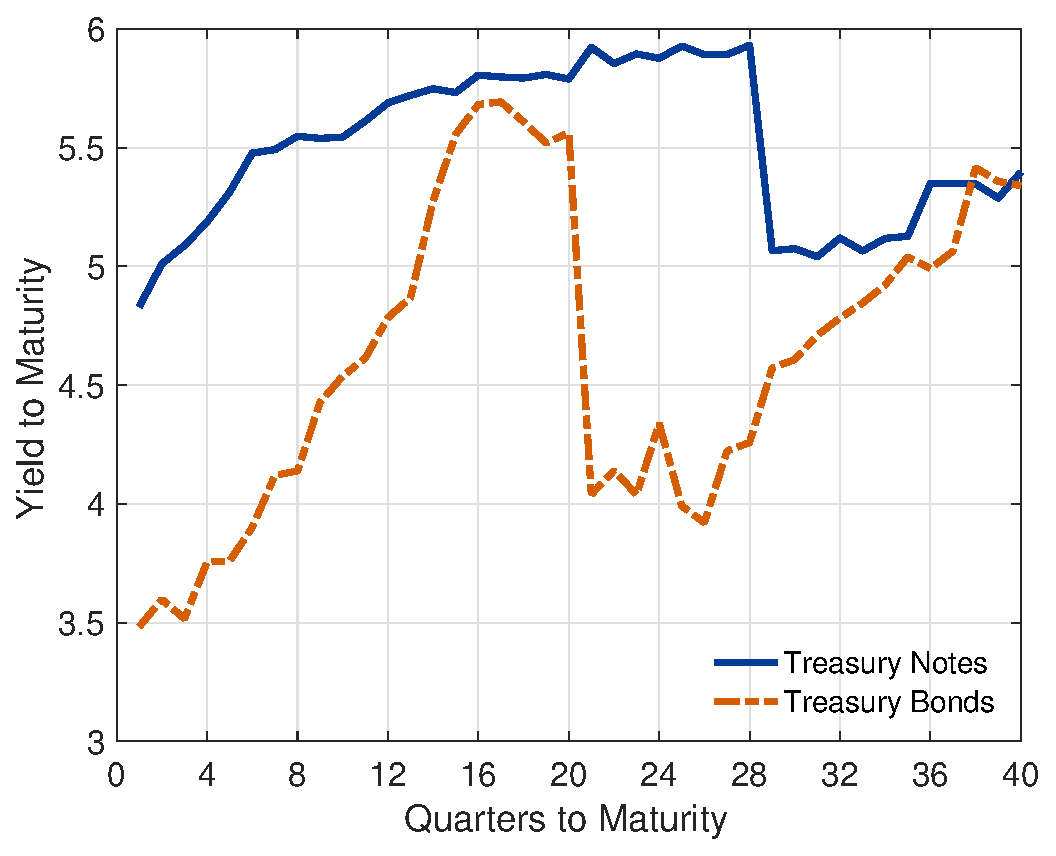
\includegraphics[width=0.7\textwidth]{BondNote_Spread.eps}
\caption{Median Treasury Bond and Note Yields with Same Time to Maturity}{(1970-2020)}
\label{fig:YTM_Spread}
\end{figure}
%: Median YTM Time Series
\begin{figure}[p]
\centering
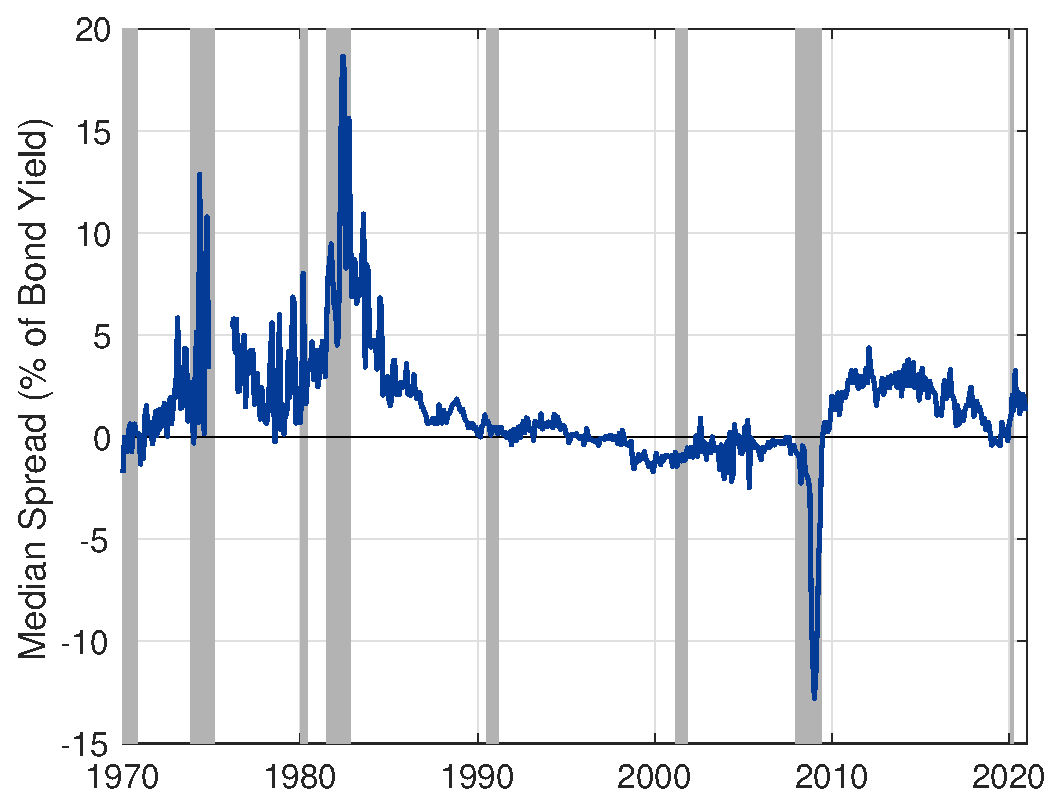
\includegraphics[width=0.7\textwidth]{BondNote_TimeSeries.eps}
\caption{Median Treasury Note--Bond Yield Spread with Same Time to Maturity}{(1970-2020)}
\label{fig:YTM_SpreadTS}
\end{figure}
%: Median Bid-Ask Spread over the Sample Period 
\begin{figure}[h]
\centering
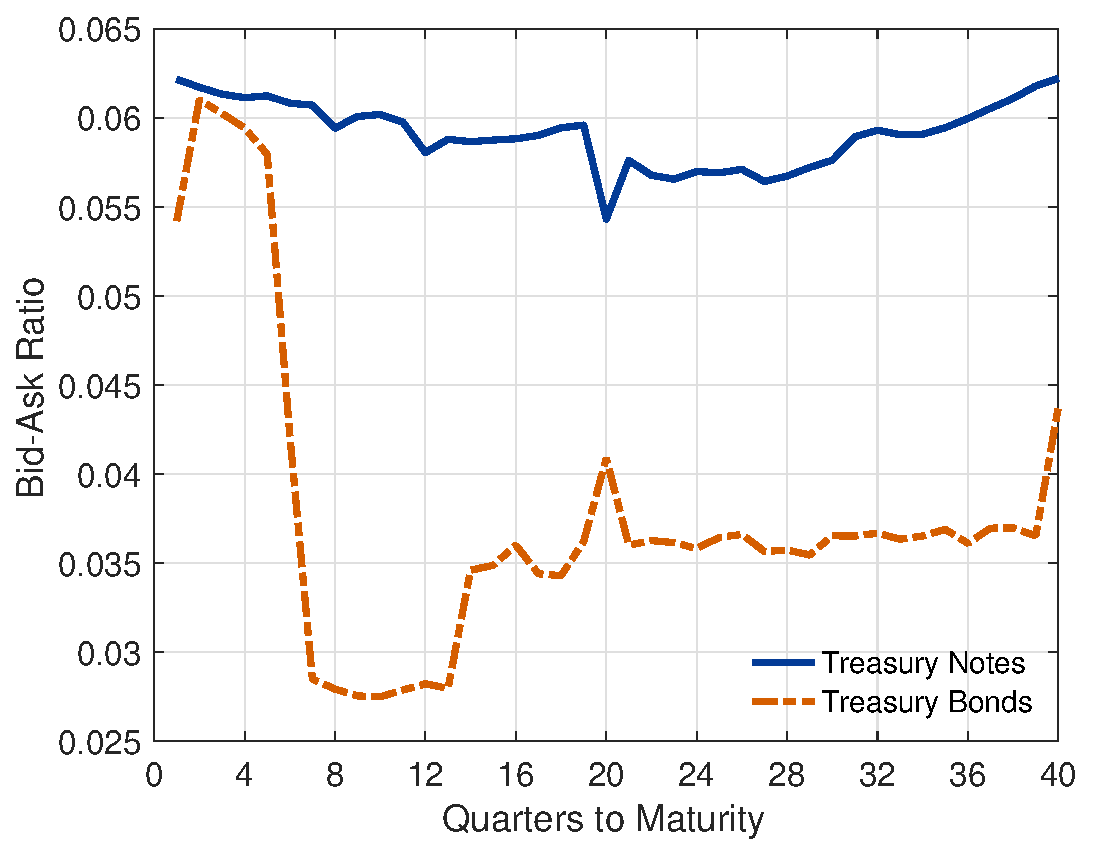
\includegraphics[width=0.7\textwidth]{BidAsk_Ratios.eps}
\caption{Median Treasury Bond and Note Bid-Ask Ratios with Same Time to Maturity}{(1970-2020)}
\label{fig:BidAsk_Ratios}
\end{figure}


\subsection{Hurdles in the Application}
\label{subsec:Hurdles}
One drawback of the T\"{o}rnqvist-Theil Divisia index is that it does not handle assets coming into and out of the market ($x_{j,t} = 0$ for some $t$) very well.
When calculating general monetary aggregates, this problem does not arise very often and is managed by imputing a reservation price and switching to a Fisher ideal index for those time periods.
Given the frequent changes in Treasury policy and the categorization I use, zero values are commonplace in this analysis.

To better account for zero values, I utilize the Fisher ideal index for the full sample.
This index still utilizes the user cost approach discussed above and is shown to be a Diewert-superlative index number like the Divisia index \citep{Diewert:1976}; but happens to be more applicable to the constraints of this particular dataset.
The Fisher ideal index (in levels) is expressed as
	\begin{equation}
		M^f_t = M^f_{t-1}\left[\frac{(\boldsymbol \eta_t \mathbf{m'}_t) (\boldsymbol \eta_{t-1} \mathbf{m'}_t)}{(\boldsymbol \eta_t \mathbf{m'}_{t-1}) (\boldsymbol \eta_{t-1} \mathbf{m'}_{t-1})}\right]^{\frac{1}{2}},
		\label{eq:FisherIdeal}
	\end{equation}
where $M^f_t$ denotes the new aggregate and the rest of the notation is defined above.
Since there is no initial value of this index $M^f_0$, the aggregate is first calculated in growth rates and then converted to a quantity index. 

\section{Theory}
\label{sec:Theory}
As \citet{Barnett:1980} outlines, aggregation theory relies on known, exact functional forms with estimable parameters.
The functions of interest are typically utility and production functions, which are often impossible to know.
This is why I rely on statistical index numbers, whose theory only relies on the existence of maximizing behavior.
From this optimizing behavior we can derive the user costs of the underlying components and bypass the unknown parameters because the resulting index numbers are not dependent on any specialized properties of the aggregator function.
That is, while I'm not deriving the true aggregate itself, the resulting quantity index will track the true aggregate.
A complete guide to index number theory and its application to monetary aggregation can be found in \citet{Barnett-Serletis:2000}.

A proper quantity index requires a price that is derived from an optimizing agent.
Thus, motivating the measurement of marketable government debt requires a partial equilibrium model that derives both the period-by-period user cost of holding government debt as well as the budgetary constraints the fiscal authority encounters.
This model incorporates both short- and long-term debt issued by the government, as well as an alternative long-term asset that will act as the benchmark asset. 
In this model, I refer to the alternative asset as ``capital,'' though it could also be motivated in some other fashion. 

\subsection{Long-Term Asset Dynamics}
The long-term government bonds and capital both evolve in a similar fashion.
As described by \citet{Krause-Moyen:2016}, each period new nominal long-term government bonds $B^{L,n}_t$ are issued, which are added to the stock of outstanding long-term debt $B^L_t$.
A portion $\alpha \in (0,1)$ of the previous period's stock of long-term bonds mature, while the remaining $(1-\alpha)$ remain in the stock of outstanding long-term debt. 
The maturity of these bonds is therefore $\sfrac{1}{\alpha}$.
Together, the stock of outstanding long-term debt evolves such that 
\begin{equation}
	B^L_t = (1-\alpha)B^L_{t-1} + B^{L,n}_t.
	\label{eq:LoM_DebtLevel}
\end{equation}
The average nominal interest rate paid on the stock of outstanding long-term debt $r^L_t$ evolves such that
\begin{equation}
	r^L_t B^L_t = (1-\alpha)r^L_{t-1}B^L_{t-1} + r^{L,n}_tB^{L,n}_t,
	\label{eq:LoM_DebtReturn}
\end{equation}
where $r^{L,n}_t$ is the interest rate on newly-issued long-term bonds. 

Capital is structured in a similar fashion, with the total stock of outstanding capital evolving according to
\begin{equation}
	K_t = (1-\delta)K_{t-1} + I_t,
	\label{eq:LoM_CapLevel}
\end{equation}
where $I_t$ is new investment in capital and $\delta \in (0,1)$ designates the portion of the outstanding stock of capital that matures each period.
This implies that the maturity of capital is $\sfrac{1}{\delta}$. 
The average interest rate paid on the capital stock outstanding $R_t$ is derived by
\begin{equation}
	R_tK_t = (1-\delta)R_{t-1}K_{t-1} + R^n_tI_t,
	\label{eq:LoM_CapReturn}
\end{equation}
where $R^n_t$ is the interest rate on newly-issued capital.

\subsection{Representative Household}
The representative household in this model works $l_t$ hours each period for nominal wage $W_t$, less an income tax rate $\tau_t$.
It also earns income through it's previous investments in capital $(\delta + R_{t-1})K_{t-1}$, short-term (one-period) bonds $(1+r_t)B_{t-1}$, long-term bonds $(\alpha + r^L_{t-1})B^L_{t-1}$, and profits from a continuum of intermediate goods-producing firms $\int^1_0 \Pi_t(s) \mathrm{d}s$.\footnote{
	The $\delta$ considered here can deviate from that in (\ref{eq:LoM_CapLevel}) if depreciation is considered.
	In this present study, however, we assume zero deprecation and treat ``capital'' as an alternative long-term security similar to the long-term government bond.
	Additionally, the inclusion/exclusion of the corporate profit term does not alter the results of this partial equilibrium setup, but would be needed in a full, general equilibrium presentation.}
This income is spread between a real consumption good $c_t$ at price $p_t$ as well as new investments in nominal short-term bonds $B_t$, long-term bonds $B^{L,n}_t$, and capital $I_t$.
Combined, the household's period-by-period budget constraint can be expressed as
\begin{multline}
	B_t + B^{L,n}_t + p_tc_t + I_t = (\delta + R_{t-1})K_{t-1} + (1+r_{t-1})B_{t-1} + \\ (\alpha + r^L_{t-1})B^L_{t-1} + (1-\tau_t)W_tl_t + \int^1_0\Pi_t(s)\text{d}s.
	\label{eq:HH_Budget}
\end{multline}

The household objective is to maximize utility over the real consumption good, the real monetary services provided by its portfolio of government bonds, and leisure
\begin{equation}
	\max\mathbb{E}_t\! \sum^\infty_{t=0} \beta^t\left\{u(c_t) + v\left(\frac{M_t}{P_t}\right) + x(1-l_t)\right\},
	\label{eq:HH_Utility}
\end{equation}
where $u(\cdot)$, $v(\cdot)$, and $x(\cdot)$ are increasing, concave functions. 
The monetary services provided by the portfolio are captured by a constant elasticity of substitution function 
\begin{equation}
	M_t = \left[\lambda^{\frac{1}{\sigma}}B_t^{\frac{\sigma-1}{\sigma}} + (1-\lambda)^{\frac{1}{\sigma}}{B^L_t}^{\frac{\sigma-1}{\sigma}}\right]^{\frac{\sigma}{\sigma-1}},
	\label{eq:HH_MonServices}
\end{equation}
where $\lambda \in [0,1]$ dictates the weight of each government debt security and $\sigma$ dictates the elasticity of substitution between the two assets.

Solving the household's problem results in the following dynamic conditions:
\begin{equation}
	1 - \gamma_{2,t}\left(\frac{\lambda M_t}{B_t}\right)^\frac{1}{\sigma} = \beta \mathbb{E}_t\!\left[\frac{\mu_{1,t+1}}{\mu_{1,t}}\frac{1+r_t}{\pi_{t+1}}\right],
	\label{eq:HH_manOC_B}
\end{equation}
%
\begin{multline}
	1 - \gamma_{2,t}\left(\frac{(1-\lambda)M_t}{B^L_t}\right)^\frac{1}{\sigma} + \gamma_{4,t}\left(r^L_t-r^{L,n}_t\right) \\
	= \beta \mathbb{E}_t\!\left[\frac{\mu_{1,t+1}}{\mu_{1,t}}\frac{1}{\pi_{t+1}} \left\{ 1+r^L_t + (1-\alpha)\gamma_{4,t+1} \left(r^L_t-r^{L,n}_{t+1}\right)\right\}\right],
	\label{eq:HH_manOC_BL}
\end{multline}
%
and
\begin{equation}
	1 + \gamma_{3,t}\left(R_t - R^{n}_t\right)  = \beta\mathbb{E}_t\!\left[\frac{\mu_{1,t+1}}{\mu_{1,t}}\frac{1}{\pi_{t+1}}\left\{ 1 + R_{t} + (1-\delta)\gamma_{3,{t+1}}\left(R_{t} - R^{n}_{t+1}\right)\right\}\right],
	\label{eq:HH_manOC_K}
\end{equation}
The solution technique to the household's problem can be found in Appendix \ref{app:HH_Solution}.
Here, $\mu_{1,t} = u'(c_t)$, $\gamma_{2,t} = \sfrac{v'(\cdot)}{u'(\cdot)}$, and $\gamma_{3,t}$ and $\gamma_{4,t}$ are the prices of the long-term assets $B^L_t$ and $K_t$, respectively.
These prices evolve according to
\begin{equation}
	\gamma_{3,t} = \beta\mathbb{E}_t\!\left[\frac{\mu_{1,t+1}}{\mu_{1,t}}\frac{1}{\pi_{t+1}} \left\{1 + (1-\delta)\gamma_{3,{t+1}}\right\}\right],
	\label{eq:HH_manOC_R}
\end{equation}
%
and
\begin{equation}
	\gamma_{4,t} = \beta\mathbb{E}_t\!\left[\frac{\mu_{1,t+1}}{\mu_{1,t}}\frac{1}{\pi_{t+1}} \left\{1 + (1-\alpha)\gamma_{4,{t+1}}\right\}\right].
	\label{eq:HH_manOC_rL}
\end{equation}

The user costs of the short- and long-term bonds are 
\begin{equation}
	\eta_t = \frac{\mathbb{E}_t \Big[ \frac{\mu_{t+1}}{\mu_{t}}\frac{1}{\pi_{t+1}} \Big\{ R^n_t - (1-\delta)\gamma_{3,t+1}\Delta R^n_{t+1} - r_t \Big\}\Big]}{\mathbb{E}_t \Big[ \frac{\mu_{t+1}}{\mu_{t}}\frac{1}{\pi_{t+1}} \Big\{ 1+ R^n_t - (1-\delta)\gamma_{3,t+1}\Delta R^n_{t+1}\Big\}\Big]},
\end{equation}
and
\begin{equation}
\eta^L_t = \frac{\mathbb{E}_t \Big[ \frac{\mu_{t+1}}{\mu_{t}}\frac{1}{\pi_{t+1}} \Big\{ R^n_t  - (1-\delta)\gamma_{3,t+1}\Delta R^n_{t+1} - r^{L,n}_t + (1-\alpha)\gamma_{4,t+1}\Delta r^{L,n}_{t+1}\Big\}\Big]}{\mathbb{E}_t \Big[ \frac{\mu_{t+1}}{\mu_{t}}\frac{1}{\pi_{t+1}} \Big\{ 1+ R^n_t - (1-\delta)\gamma_{3,t+1}\Delta R^n_{t+1}\Big\}\Big]},
\label{eq:usercost_LT}
\end{equation}
respectively.
The derivations of these user costs can be found in Appendix \ref{app:usercost_derivation}.

\subsection{Fiscal Capacity Considerations}
\label{subsec:Theory_Capacity}
\citet*{Brunnermeier-Merkel-Sannikov:2022} have shown that government debt constraints need to be augmented for the service flows (transaction/monetary services) that the securities provide.
Here I expand upon this idea with the specifics of the model above, providing a deeper look at how we can ascertain those services flows in particular.\footnote{
	This is identical to the exercise conducted by \citet{Brunnermeier-Merkel-Sannikov:2020}, though I abstract from the bubble term to focus solely on the monetary services component.}
Consider the simple budget constraint of the government in this model
\begin{equation}
	(1+r_{t-1})\frac{B_{t-1}}{p_t} + (\alpha + r^L_{t-1})\frac{B^L_{t-1}}{p_t} = \frac{B_t}{p_t} + \frac{B^{L,n}_t}{p_t} + s_t,
\end{equation}
where $s_t$ is denotes the real primary surplus. 
Now incorporate (\ref{eq:LoM_DebtLevel}) into the above equation to get
\begin{equation}
	(1+r_{t-1})\frac{B_{t-1}}{p_t} + (1 + r^L_{t-1})\frac{B^L_{t-1}}{p_t} = \frac{B_t}{p_t} + \frac{B^{L}_t}{p_t} + s_t.
\end{equation}
Since (\ref{eq:HH_manOC_B}) and (\ref{eq:HH_manOC_BL}) must hold,
\begin{multline}
	\frac{B_{t-1} + B^L_{t-1}}{p_t}(1+r_{t-1})= s_t  - (r_{t-1}^L - r_{t-1})\frac{B^L_{t-1}}{p_t} + \beta\mathbb{E}_t\left[\frac{\mu_{1,t+1}}{\mu_{1,t}} \frac{B_{t} +B^L_{t}}{p_{t+1}}(1+r_{t})\right] \\ 
		- \beta\mathbb{E}_t\left[\frac{\mu_{1,t+1}}{\mu_{1,t}} \frac{B^L_{t}}{p_{t+1}}(1+r_{t})\right] + \beta\mathbb{E}_t\left[\frac{\mu_{1,t+1}}{\mu_{1,t}} \frac{B^L_{t}}{p_{t+1}}(1+r^L_{t})\right] \\
		+  \gamma_{2,t}\left(\frac{\lambda M_t}{B_t}\right)^\frac{1}{\sigma}\frac{B_t}{p_t} +\gamma_{2,t}\left(\frac{(1-\lambda) M_t}{B^L_t}\right)^\frac{1}{\sigma}\frac{B^L_t}{p_t} \\
		+\beta\mathbb{E}_t\left[\frac{\mu_{1,t+1}}{\mu_{1,t}} \frac{B^L_t}{p_{t+1}}\left\{1+  (1-\alpha)\gamma_{4,t+1}\left(r^L_t - r^{L,n}_{t+1}\right)\right\}\right] - \gamma_{4,t}\left(r^L_t - r^{L,n}_t\right)\frac{B^L_t}{p_t}
\end{multline}
Including (\ref{eq:HH_manOC_rL}) and some rearranging, we can simplify the above equation to
\begin{multline}
	\frac{B_{t-1} + B^L_{t-1}}{p_t}(1+r_{t-1})= s_t - (r_{t-1}^L - r_{t-1})\frac{B^L_{t-1}}{p_t} + \beta\mathbb{E}_t\left[\frac{\mu_{1,t+1}}{\mu_{1,t}} \frac{B_{t} +B^L_{t}}{p_{t+1}}(1+r_{t})\right] \\ 
		+ \beta\mathbb{E}_t\left[\frac{\mu_{1,t+1}}{\mu_{1,t}} \frac{B^L_{t}}{p_{t+1}}(1+r^L_{t} - (1-\alpha)\gamma_{4,t+1}\Delta r^{L,n}_{t+1} - r_t)\right]  \\
		+  \gamma_{2,t}\left(\frac{\lambda M_t}{B_t}\right)^\frac{1}{\sigma}\frac{B_t}{p_t} +\gamma_{2,t}\left(\frac{(1-\lambda) M_t}{B^L_t}\right)^\frac{1}{\sigma}\frac{B^L_t}{p_t}.
\end{multline}

The last two terms are of particular importance here.
Incorporating the definition of the monetary services aggregate reduces the above expression to 
\begin{multline}
	\frac{B_{t-1} + B^L_{t-1}}{p_t}(1+r_{t-1})= s_t  - (r_{t-1}^L - r_{t-1})\frac{B^L_{t-1}}{p_t} + \beta\mathbb{E}_t\left[\frac{\mu_{1,t+1}}{\mu_{1,t}} \frac{B_{t} +B^L_{t}}{p_{t+1}}(1+r_{t})\right] \\ 
		+ \beta\mathbb{E}_t\left[\frac{\mu_{1,t+1}}{\mu_{1,t}} \frac{B^L_{t}}{p_{t+1}}(1+r^L_{t} - (1-\alpha)\gamma_{4,t+1}\Delta r^{L,n}_{t+1} - r_t)\right] 
		+  \gamma_{2,t}\frac{M_t}{p_t},
	\label{eq:fiscalcapacity}
\end{multline}
where it can be shown that
\begin{equation}
	\gamma_{2,t} = \left[\lambda \eta_t^{\sigma-1} + (1-\lambda)\left(\eta^L_t\right)^{\sigma-1}\right]^\frac{1}{\sigma-1}
	\label{eq:price_dual}
\end{equation}
is the price dual for the monetary services aggregate. 

There are a couple of items to point out with regards to the above expression.
First, fiscal capacity intuitively diminishes as long-term rates rise relative to short-term rates.
This term is reflecting the convenience yields that the government enjoys on its short-term debt.
Second, the fourth term on the right side suggests long-term debt can improve fiscal capacity via its longer maturity and a higher expected one-period return over the short-term debt. 
That is, while capacity shrinks with higher long-term interest rates, demand for the debt increases with higher expected holding-period returns. 
Lastly, fiscal capacity increases with the value of the monetary/transaction services the debt provides.
Thus, the monetary services provided by government debt issuances is directly captured in the government's budget constraint in a similar fashion to that shown in \citet{Brunnermeier-Merkel-Sannikov:2022}.


\section{Data and Methodology}
\label{sec:DataMethodology}
In this section, I construct the Fisher ideal quantity index described in Section \ref{sec:Theory} from data compiled by the Center for Research in Securities Prices on marketable Treasury securities.
Non-marketable debt is typically held by intergovernmental agencies, and is therefore not typically considered to be a significant burden.\footnote{
	The inclusion of only publicly-held, marketable US Treasury debt would be the optimal choice here, but data restrictions keep me from assessing this.
	For instance, the CRSP data doesn't include the amount of each T-bill issuance held publicly.
	Another option could be to exclude the issuances held by the Federal Reserve, since that is the primary non-public holder of US Treasuries, but the SOMA data only goes back to 2003.
	Future research could apply this methodology to the shortened timeframe.}
The Treasury began its ``regular and predictable'' debt issuance campaign in the 1970s and data regarding the spot and forward interest rates goes back to January 1977.
Therefore the variables constructed here will cover the February 1977 to December 2020 period.

The first issue that needs to be addressed is essentially analogous to new-product bias.
As (\ref{eq:FisherIdeal}) shows, the calculation of the growth rates requires both current and lagged quantities and user costs. 
If I were to treat each issuance as a separate $m_{i,t}$, there would be distortions at issuance and maturity months.
For example, in the issuance month of $m_{i,t}$, the preceding month's yield $r_{i,t-1}$ of that particular issuance doesn't exist, which means its user cost $\eta_{i,t-1}$ also doesn't exist.
Therefore, an assumption would need to be made regarding this lagged user cost.
\citet{Feenstra:1994} and others have outlined a theoretically justified solution to this problem in which the price is set at its reservation level, where the quantity demanded would equal zero in the preceding month.\footnote{
	The Center for Financial Stability, which publishes data on Divisia monetary aggregates, delays the inclusion of new monetary assets for a few months.
	In this situation, however, the regular issuance and maturity of short-term debt make this strategy problematic.}
It's also well documented that on-the-run bonds sell at a premium over their off-the-run counterparts, suggesting $\eta_{i,t-1} > \eta_{i,t}$, but by how much?
Estimating the reservation price of each issuance in each month over the sample period would seem to be too technically burdensome. 
With how distortionary this bias can be, some adjustments and/or assumptions are needed.

To reduce the magnitude of this issue, I cluster the assets into groups that are most likely to be perfect substitutes in any given month.
While there may be discrepancies in on-the-run/off-the-run securities, they should average out within the clusters. 
Based on the work of \citet{Amihud-Mendelson:1991} as well as the descriptive statistics in Figures \ref{fig:YTM_Spread} and \ref{fig:BidAsk_Ratios}, the securities need to be separated across their designation of {\em bills}, {\em notes}, and {\em bonds}.
Since 1997, the Treasury has issued Treasury Inflation-Protected Securities (TIPS), which yield a real rate of interest instead of the traditional nominal yield.
These have been shown to be less liquid than their nominal counterparts, so I create two additional categories of {\em TIPS notes} and {\em TIPS bonds}. 
Lastly, as these securities mature, their yields tend to fall with the trend of the constant maturity yield curve, reflecting the changing monetary services they provide.
Therefore, each of these five categories needs to be further segmented by their time to maturity.
Since bonds and longer notes are issued on a quarterly basis, it's common to have individual months where there are no securities of a certain type.\footnote{
	These notes and bonds are typically subject to reopenings in the months following the initial issuance, but the maturity dates are unchanged.
	For example, if a 30-year bond is issued in February, a reopening of that issuance may be offered in March, but the time-to-maturity on that reopening is 29 years, 11 months.}
A fine-grained segmentation such as this would again be subject to a large amount of new-product bias, so I define each sub-category as the quarters-to-maturity.
That is, for securities that will mature over the next one-to-three months, they are categorized has maturing within one quarter. 
A thirty-year threshold on bonds suggests 120 quarters-worth of categories, but there were a series of longer-term bonds that were issued between 1953 and 1965, which could impact the first years of the analysis.
Therefore, the number of quarters-to-maturity categories is set at 160, or forty years. 
Overall, when accounting for both the types of securities and the quarters to maturity, there are 800 categories.\footnote{
	Note that, based on (\ref{eq:FisherIdeal}), baskets that are consistently empty do not impact the measurement, allowing me to keep it consistent across the types of securities.
	So while there are 800 total baskets, a large number of them will not contribute to the measurement, but it does provide the flexibility needed for the aggregate over the almost fifty-year analysis.}
	
The next step in this process is to identify the proper interest rates from the theory above.
Since the user costs represent the holding period return and incorporate the interest rates paid on newly-issued securities ($r_t$ and $r^{L,n}_t$) and not on the average interest rate paid out on outstanding debt ($r^L_t$), the most accurate interest rates to consider are the coupon rates.
Additionally, the term $(1-\alpha)\gamma_{4,t+1}\Delta r^{L,n}_{t+1}$ represents the expected capital gains of the long-term bond. 
To account for these expectations, I use the current price of the bonds adjusted for its maturity, multiplied by the difference between the one-month-ahead forward rate and spot rate for each bond's particular month and maturity.
For TIPS, I consider the real spot and forward yield curves in the calculation of expected capital gains. 
While forward rates incorporate more than just future expectations of current spot rates, the impact of any term premium looking only one month ahead should be negligible.

The rate considered for each basket of securities is the quantity-weighted average over the issuances therein, though a further assumption is needed to address missing values/new-product bias.
As discussed above, even the broader categories used here do not ensure that there are no issues with new-product bias.
Since most of the empty categories in this situation are simply a cluster of maturing debt through time, and not new issuances of debt, I use the linear interpolation of the rates across the maturities instead of calculating a reservation rate.
This ensures that I'm capturing the true shape of the yield curves used. 

The benchmark rate used here is the maximum holding-period return of the baskets of securities considered each month, plus twenty-five basis points.\footnote{
	Previous iterations of this measurement attempted to use the Baa Corporate Bond yield, which would have accounted for both the liquidity and safety attributes of Treasury securities.
	However, even the addition of 200 basis points did not ensure that all user costs were positive across the sample period, especially in the volatile years of 1979--1981 and long periods of time between 2014 and 2016.
	Adjustments to create that kind of spread for the early years also had the drawback of washing out the differences in user costs in the later parts of the sample period.}
This is similar to the strategy used by the Federal Reserve in their calculation of Divisia monetary aggregates and is common in other derivations of user costs. 

\section{Results}
\label{sec:Results}

\subsection{The Measure}
\label{subsec:Results_Measure}

The month-over-month growth rates of both the true aggregate and its simple sum counterpart are constructed from the data.
This indirect approach to the aggregates' levels is necessary as there is no initial value from which to begin the calculation of (\ref{eq:FisherIdeal}).
Simply taking the logarithm of (\ref{eq:FisherIdeal}) yields the growth-rate variation used.
The general levels of the growth rates are similar, so I present their spread in Figure \ref{fig:Growth_Spread}.
To aid in the visual analysis, the 12-month moving average (centered on the seventh month) spread of these growth rates is superimposed.
As can be seen, the true aggregate tends to grow faster than the simple sum aggregate, but there are also periods of relatively slow growth.
%: Differences in the Aggregates' Growth Rates
\begin{figure}[h]
\centering
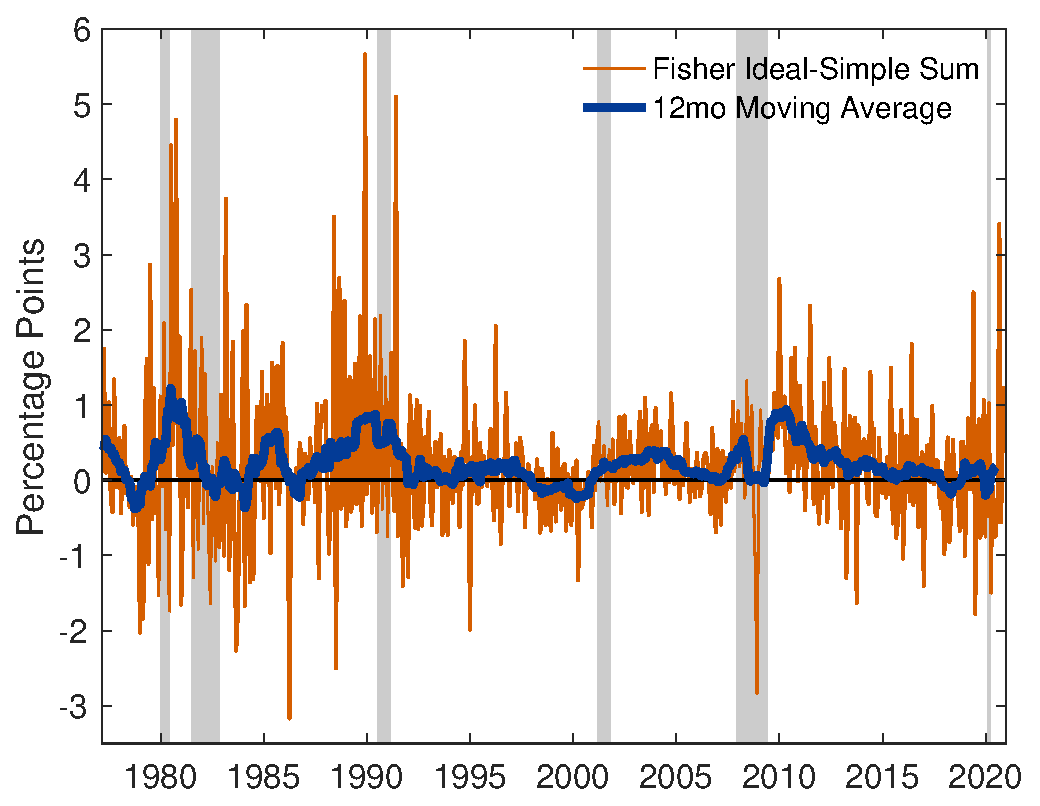
\includegraphics[width=0.85\textwidth]{GrowthDiff_v2.eps}
\caption{Month-over-month Growth Rate Spread}
\label{fig:Growth_Spread}
\end{figure}

Since the true aggregate incorporates both the quantities of the underlying assets and the monetary services they provide, the spread intuitively reveals the growth of these monetary services alone.
That is, I am essentially factoring-out the growth that comes purely from the issued principal values.
The spread in Figure \ref{fig:Growth_Spread}, therefore, represents the growth of fiscally-provided monetary services.
This figure shows us that the Treasury generally adds to the stock of monetary services over time, with notable exceptions in the late-1990s when the government was running a fiscal surplus.
In that instance, the growth rates suggest that the monetary services provided were shrinking along with the principal values. 


%: Index Values of the Monetary Services
\begin{figure}[h]
\centering
\includegraphics[width=0.85\textwidth]{MonetaryServices_Index.eps}
\caption{Monetary Services Level}
\label{fig:MS_Index}
\end{figure}
Using these growth rate spreads, I derive an index that tracks the stock of monetary services, shown in Figure \ref{fig:MS_Index}.
Multiple theories have claimed that Treasury securities provide services above and beyond their principal value, but this is the first attempt to measure such services. 
The base month considered here is August 1989 due to the relative flatness of the yield curve at that time.
When the yield curve is flat, the differences in the user costs are minimal, suggesting that the underlying assets are perceived as near-perfect substitutes and collapsing the Fisher ideal index into a simple sum aggregate.

\subsection{What Services do Treasury Securities Provide?}
\label{subsec:MonetaryServices}
The motivation and theory developed above claims that the Treasury provides monetary services above and beyond the sheer quantity of outstanding principal values, but does not take a stand on where those services originate or what they definitively represent.
These types of measurements, by definition, cannot separate one service from another.
Since the model does not separate liquidity from safety, in this section I explore empirically what services the Treasury's portfolio is actually providing.

To assess which services are provided by the Treasury, I use \citet{Jorda:2005} projections to estimate the impact of an increase in these measured monetary services on the price of safety and liquidity.\footnote{
	The potential collateral services provided by US Treasury securities is assessed in Appendix \ref{app:MonetaryServices}.}
This is in a similar vein to the work of \cite{Krishnamurthy-VissingJorgensen:2012} and others to study the impact of increased debt levels on the financial market attributes.

\paragraph{Identification of Exogenous Shocks}
The monetary services supplied by these marketable US Treasury securities are likely to be highly sensitive to general financial shocks and market perception/expectations.
Thus, identifying shocks starts with controlling for the sources of these changes. 
Exogenous shocks to the level of monetary services $m_t$ shown in Figure \ref{fig:MS_Index} are identified using a simple OLS forecasting approach
\begin{equation}
	m_t = c + \Gamma(L)X_t + \epsilon_t,
	\label{eq:Shock_ID}
\end{equation}
where $c$ is a constant term and $X_t$ are the independent variables that most likely contribute to external fluctuations in these monetary services.
To eliminate fluctuations stemming from the overall macroeconomic environment, I include the Wilshire 5000 stock index and the 10-year, 2-year yield curve spread.
The monthly standard deviation of the respective daily Wilshire 5000 stock index values controls for external variations in financial market safety and proxies for overall default risk as in \citet{Krishnamurthy-VissingJorgensen:2012}.
The level of the simple sum aggregate as well as lagged values of the constructed stock of monetary services provided are included to control for general stock and auto-regressive effects. 
Lastly, the monetary services provided by the US Treasury are likely to be relative to those of other advanced economies, with the Euro debt crisis in the 2010s serving as a key example. 
Including the trade-weighted US dollar index (major currencies) should provide a good proxy to variations stemming from these relative changes.\footnote{
	This particular variable was discontinued at the end of 2020 and was replaced with the nominal advanced foreign economies US dollar index.
	In the overlapping months---adjusting for the different index years---their variations are nearly identical.
	Therefore, the dollar index used in this analysis is a combination of the two, using their average in the overlapping months.}
All variables are in nominal form and are monthly in frequency.
Four lags of these independent variables are considered based on AIC. 
The residuals $\epsilon_t$ are taken as the estimated exogenous shocks to the stock of fiscal monetary services.

\paragraph{Estimation of the Financial Attributes}
Impulse response functions are estimated via the linear function
\begin{equation}
	z_{t+h} = c_t + \Phi(L_h)y_t + \beta_h\epsilon_t + \varepsilon_{t+h},
	\label{eq:Jorda_Model}
\end{equation}
where $h$ is the forecast horizon, $z_{t+h}$ is the dependent variable, $\epsilon_t$ is the identified shock of choice, $y_t$ is the vector of control variables including lags of up to $L_h$, and $\beta_h$ form the estimated impulse response functions.
The variable $c_t$ is a vector of trends including the constant term as well as time trends ranging from linear to fourth-order.

For this exercise, there are two dependent variables of interest: the spread between the Baa and Aaa corporate bond yields, which proxies as a safety premium, and the spread between the Aaa corporate bond yield and the 10-year Treasury constant maturity rate, which proxies as a liquidity premium.\footnote{
	Availability of the Baa corporate bond yield restricts the period to 1986:01--2021:12, which consists of 420 observations before lags are considered.}
The independent variables $y_t$ in the model include the derived measurement, the simple-sum aggregate of outstanding principal values, the 10-year/3-month yield curve spread, the equity market volatility tracker, the monetary base, and dummy variables representing recessions and the zero-lower bound.
As one cannot rule out the interdependence of liquidity and safety in asset markets, lags of both interest rate spreads are included in each as an attempt to control for this possibility.
All variables are in nominal form and are monthly in frequency.
A horizon of eighteen months is considered, lags are chosen at each horizon by AIC with maximum number of lags set at twelve, and Newy-West standard errors are used. 

%: Lag structure chosen by AIC
% Safety -  10    10     7     6     7     7     6     6     6    12    12    12    11    10     9     8     7     5
% Liquidity - 9     9     1     9     8     7     6    12    12    12    12    12    12    12    12    12    12    11

%: IRF: Safety to Monetary Services Shock
\begin{figure}[p]
\centering
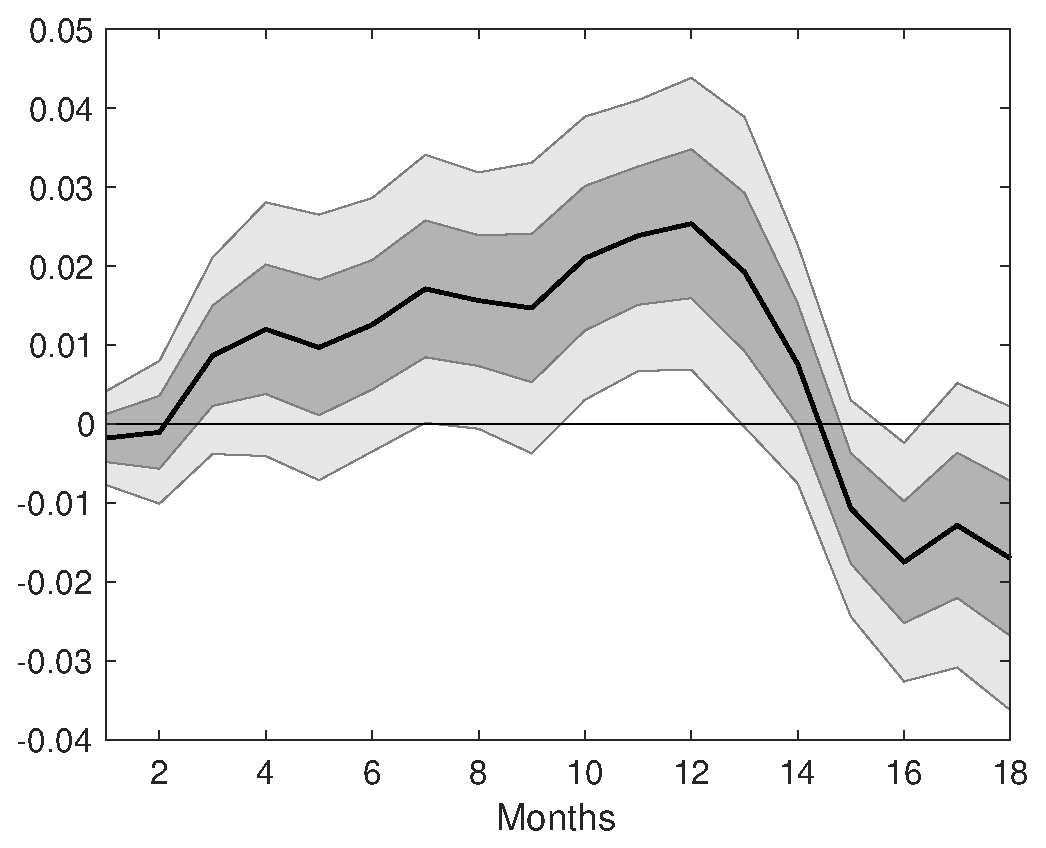
\includegraphics[width=0.7\textwidth]{Attributes_Safety.eps}
\caption{Impact of Monetary Services on Baa--Aaa Spread}
\label{fig:Attributes_Safety}
\end{figure}
%: IRF: Liquidity to Monetary Services Shock
\begin{figure}[p]
\centering
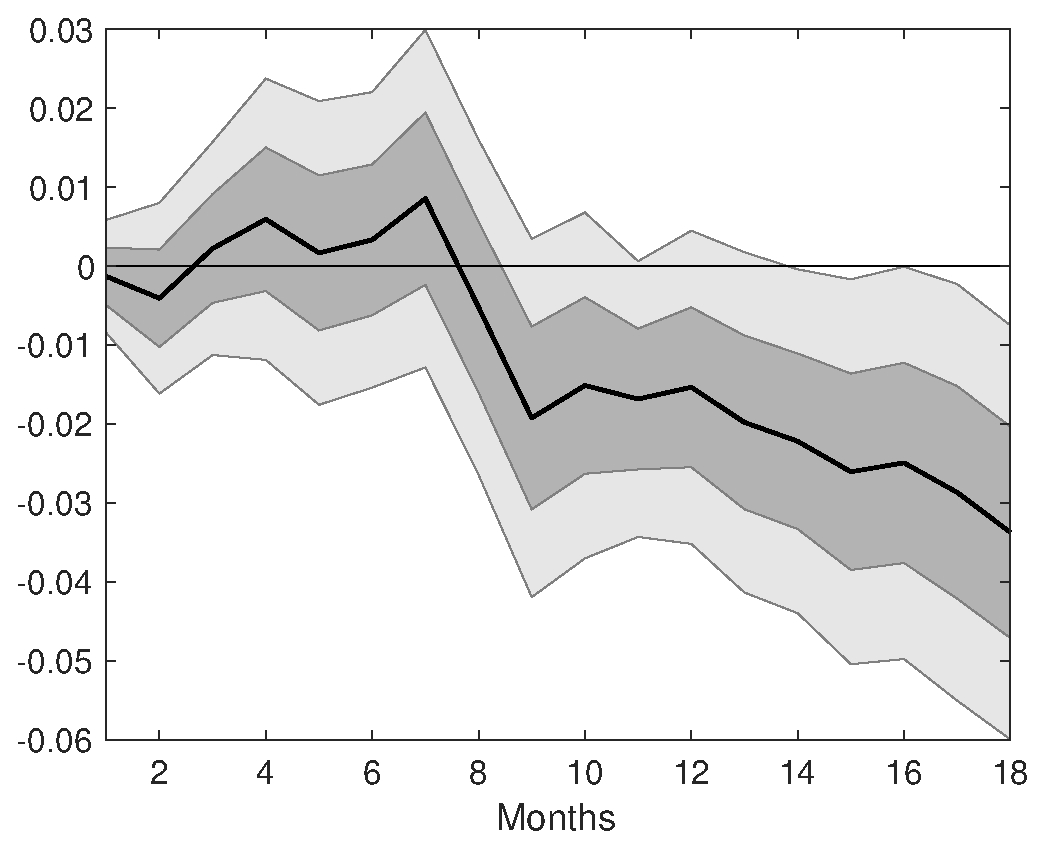
\includegraphics[width=0.7\textwidth]{Attributes_Liquidity.eps}
\caption{Impact of Monetary Services on Aaa--10yr Spread}
\label{fig:Attributes_Liquidity}
\end{figure}

The estimated response functions and their 68- and 95-percent confidence intervals are presented in Figures \ref{fig:Attributes_Safety} and \ref{fig:Attributes_Liquidity}.
The Baa--Aaa spread (Figure \ref{fig:Attributes_Safety}) increases on average in response to a unit shock to fiscal monetary services, becoming statistically significant at seven months and persistently so during the 10--12-month period. 
% becoming statistically significant at the eight-month mark and remaining elevated for approximately two months.
That is, while gradual, it causes the price of safety to fall. 
This would correspond to an increase in the supply of safe assets in the market, suggesting that safety is, indeed, one of the monetary services provided. 
Considering the point estimates and the 68-percent confidence interval, is easier to see that these safety services build over time, peaking around a year after the shock. 
This corroborates with the positive \citet{Krishnamurthy-VissingJorgensen:2012} result, though they consider annual data in their analysis and would not pick up the gradual nature of the effect.

The impact on liquidity, however, is counter-intuitive given the standard narrative.
Figure \ref{fig:Attributes_Liquidity} suggests that an increase in these monetary services has little impact on market liquidity and even leads to an increase in the price of liquidity at later horizons. 
While \citet{Krishnamurthy-VissingJorgensen:2012} find that an increase in the debt-to-GDP ratio reduces the price of liquidity in the market, my results out to a year are null. 
Given that the related, additional components in the fiscal capacity literature \citep[e.g.][]{Brunnermeier-Merkel-Sannikov:2022} are typically labeled as ``transaction services,'' this result is particularly surprising.

One potential explanation of the lack of liquidity provided by the Treasury corresponds to the line of reasoning by \citet{Singh-Stella:2021} regarding quantitative easing.
That is, issuing new bonds requires the extraction of other forms of money from the economy that are at least as liquid.
So, on net, and despite US Treasuries' enhanced liquidity features relative to other debt securities, new issuances actually reduce liquidity in the market.
This is explored further in Appendix \ref{app:MonetaryServices}, where I recalculate the aggregates and the impulse response functions after separating the portfolio into bills and notes/bonds.
I find the potential increase in liquidity due to bill issuance to not be statistically significant, while note/bond issuance reduces liquidity in the market on impact.
Thus, while I will continue to use the phrase ``monetary services" going forward for consistency, it seems that the Treasury is primarily supplying safety to the markets, not necessarily liquidity.
Further exploration of this specific point is left to future research.


\subsection{Further Analysis}
%: YoY Fiscal Monetary Services Growth
For a more intuitive and readable view of the growth rate of these monetary services, Figure \ref{fig:YoY_growth} presents the spread in the year-over-year growth rates constructed from the index in Figure \ref{fig:MS_Index}.
One of the larger and more sustained spreads in recent years came with the combination of the American Recovery and Reinvestment Act of 2009 (ARRA) and the European debt crisis from January 2009, through about April 2013. 
The additional quantity of Treasury debt, combined with the rush to safety from European bond markets caused the monetary services of the underlying Treasury debt to outgrow the pure quantity being created for a pronounced time.
%The ``dash for cash'' can also be seen during the months of the COVID recession and the months immediately following.
%This crisis can be seen as a sharp decrease in the demand for monetary services bonds provided.
The increase in monetary services can also be seen in the late-1980s and early-1990s as the savings-and-loan crisis burned through the US economy.
This measure, and the events surrounding its peaks and troughs, lend additional credence to it capturing the monetary services---particularly safety---of US Treasury debt. 
\begin{figure}[h]
\centering
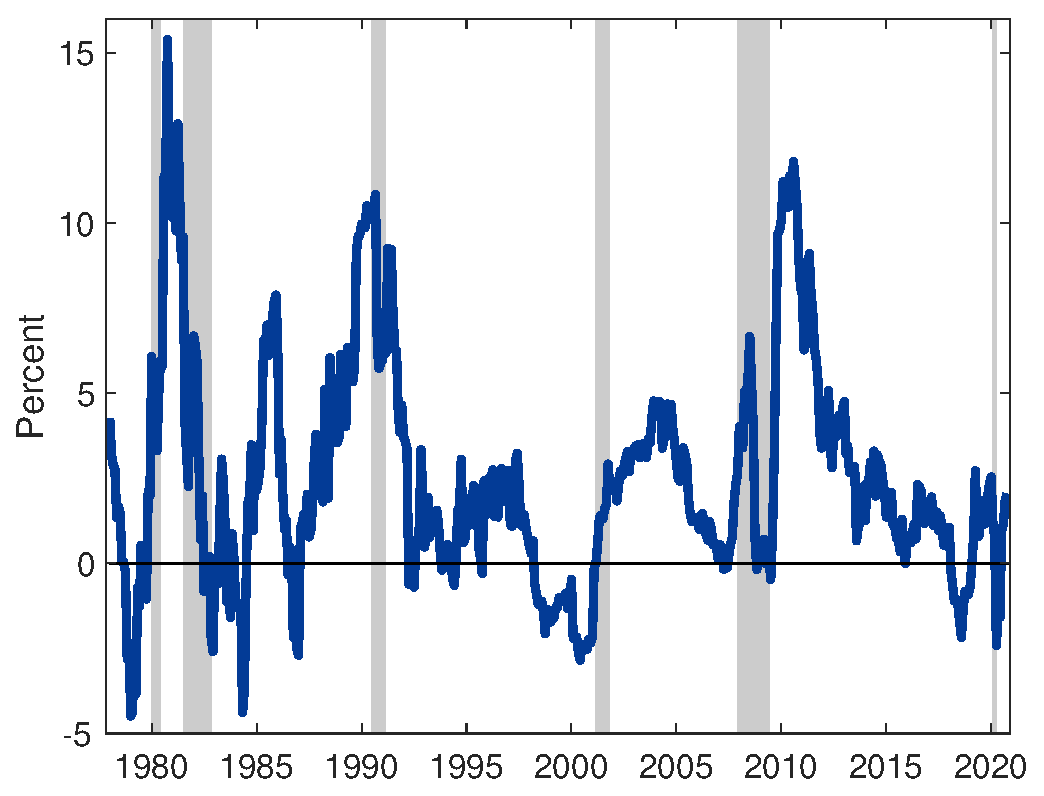
\includegraphics[width=0.85\textwidth]{YoYGrowth_MonServices.eps}
\caption{Year-over-year Growth of Fiscal Monetary Services}
\label{fig:YoY_growth}
\end{figure}
%With no initial value, derivation of the measure in is done by taking the logarithm of (\ref{eq:FisherIdeal}) and calculating the growth rate of the index.
%Figure \ref{fig:Growth_Spread} presents the spread between the month-over-month growth rates of the Fisher ideal index and its simple sum counterpart.
%Intuitively, since the Fisher ideal incorporates both the quantities and the monetary services of the underlying assets, while the simple sum is a purely quantity aggregate, the difference in their growth rates should isolate the growth rate of the monetary services of the debt.
%Since these differences in month-over-month growth rates can be rather volatile, a 12-month moving average (centered on the seventh month) is superimposed.
%This figure shows us that the Treasury generally adds to the stock of monetary services over time, with notable exceptions in the late-1990s when the government was running a fiscal surplus.
%In that instance, the growth rates suggest that the monetary services provided were shrinking along with the principal values. 
%

%The derived month-over-month growth rates can be used to create level indices that track both aggregates, which are presented in Figure \ref{fig:IndexValues}.
%%: Index Values of the Aggregates
%\begin{figure}[h]
%\centering
%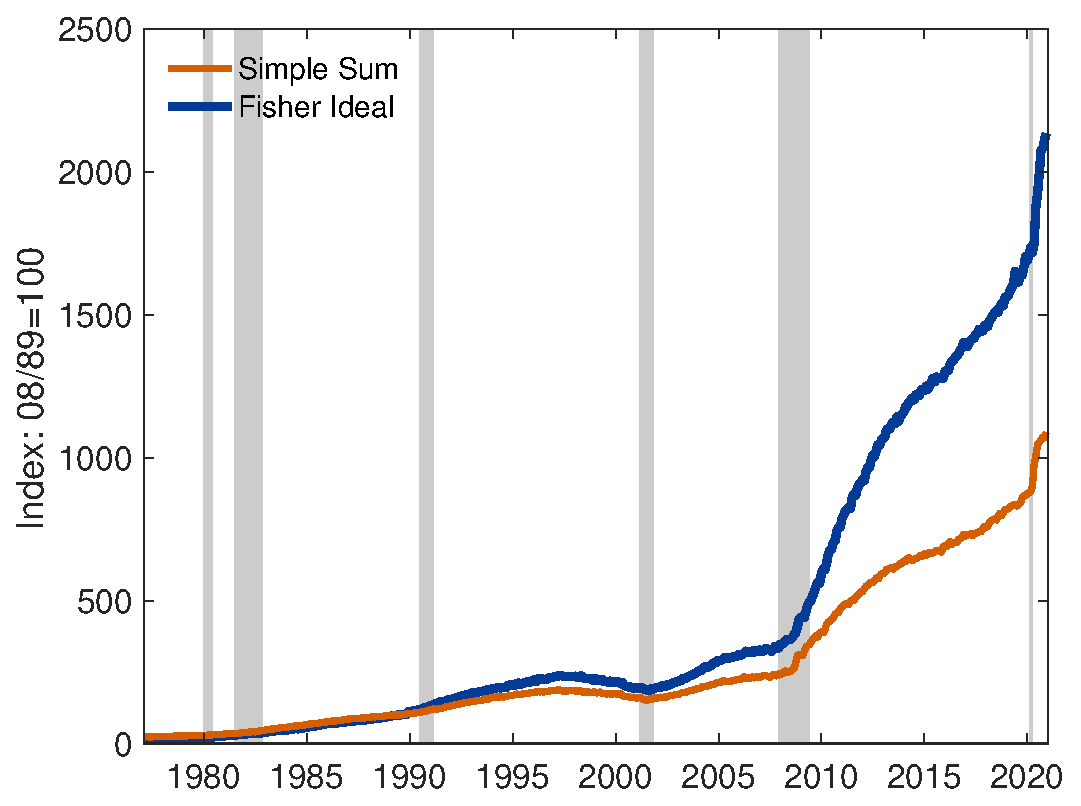
\includegraphics[width=0.7\textwidth]{FisherIndex_v2.eps}
%\caption{Fiscal Debt Level Indices}
%\label{fig:IndexValues}
%\end{figure}




\subsection{Fiscal Capacity Considerations}
\label{subsec:Results_Capacity}
In Section \ref{subsec:Theory_Capacity} I showed that the total value of the monetary services aggregate $M_t$ expands the fiscal capacity to borrow.
Incorporating the aggregate's price dual from (\ref{eq:price_dual}) provides the measure of the total value shown in Figure \ref{fig:FiscalServices_Value}.
%This measure can be found in the last term of (\ref{eq:fiscalcapacity}) as the additional fiscal capacity provided by these monetary services.
The data does not go back far enough to know whether the higher values in the late 1970s are a one-off spike or a sustained trend. 
The sudden decrease in this index in the 1989--1990 period comes from a sudden decrease in the price of obtaining these monetary services.
While the reasoning for this dramatic shift is beyond the scope of this paper, this does generally align with some later estimates of the Great Moderation as well as the surge in the information technology realm.\footnote{
	While most of the work on the Great Moderation centers around 1984:Q4 as the break point, \citet{Stock-Watson:2002} find a relatively wide 95\% confidence interval that expands all the way to 1989:Q4.
	The first web browser was also introduced in 1990, providing information in an easy-to-use format to the masses.}
One could imagine that the decrease in general market volatility, coupled with an increase in the available information about other financial assets, decimated the Treasury's comparative advantage in safety in the financial world.
\begin{figure}[h]
\centering
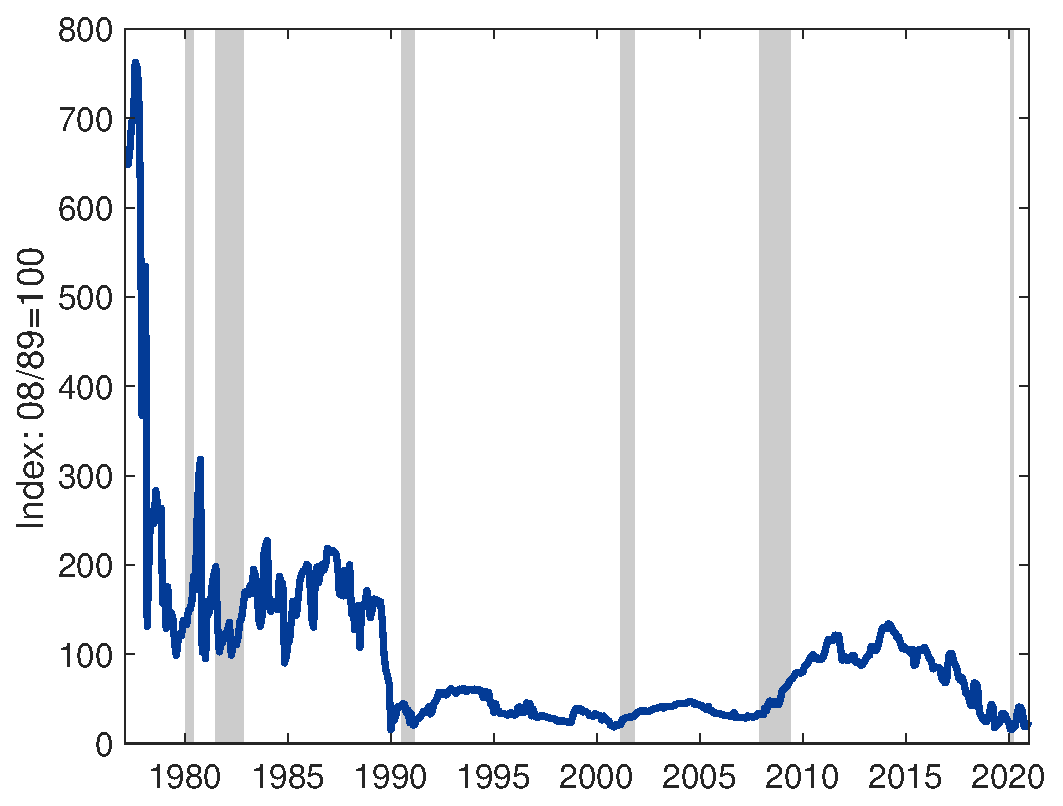
\includegraphics[width=0.85\textwidth]{FiscalCapacity_Index.eps}
\caption{Value of Fiscal Monetary Services}
\label{fig:FiscalServices_Value}
\end{figure}

The value of the monetary services aggregate was relatively stable until the financial crisis of 2007-2009, when that value increased approximately 378 percent from January 2007 to January 2014. 
This increase in the fiscal capacity would help explain the lack of inflationary pressure during that period of expansion despite increases in federal spending and monetary stimulus over that time.
The stimulus passed during the 2020 pandemic, however, did not provide the same increase in total value, as the private sector moved towards pure liquidity (``dash for cash'') in the face of lockdowns.
In that type of environment, even Treasury securities do not provided the needed liquidity and safety features.

\section{Monetary--Fiscal Interaction with Fiscal Monetary Services}
\label{sec:MonetaryFiscal}
In this section, I evaluate the impact of fiscally-provided monetary services on the interaction between monetary and fiscal policies.
To do so, I construct the rest of the small-scale New Keynesian model in a fashion similar to that of \citet{Ireland:2004} and \citet{Belongia-Ireland:2014}.
It incorporates a continuum of monopolistically competitive, intermediate goods-producing firms which face a Rotemberg cost-of-price-adjustment constraint, and a final goods-producing firm which aggregates these intermediate goods using a CES production function. 
%a fiscal authority which taxes, spends, and borrows both at short- and long-durations, and a monetary authority that sets interest rates in accordance with a Taylor rule.
The policy-side of the model is presented below, while the firm-side of the model can be found in Appendix \ref{app:Model}.

\subsection{Adjustments to the Initial Model}
The focus of the initial model in Section \ref{sec:Theory} was the proper motivation for an index number.
With the focus now on the interaction between monetary and fiscal policies, the model needs to be built-out to incorporate more applicable features.
For instance, in this section I incorporate fiat currency $F_t$ in the monetary services aggregate
\begin{equation} \tag{\ref{eq:HH_MonServices}*}
	M_t = \left[\lambda_1^{\frac{1}{\sigma}}F_t^{\frac{\sigma-1}{\sigma}} +
			\epsilon^s_t\left( \lambda_2^{\frac{1}{\sigma}}B_t^{\frac{\sigma-1}{\sigma}} + 
			 \lambda_3^{\frac{1}{\sigma}}{B^L_t}^{\frac{\sigma-1}{\sigma}}\right)\right]^{\frac{\sigma}{\sigma-1}},
	\label{eq:AltMonetaryServices}
\end{equation}
where $\lambda_1, \lambda_2, \lambda_3 \geq 0$ and $\sum_{i=1}^3 \lambda_i = 1$.
The term $\epsilon^s_t$ is the monetary services shock to the debt portfolio, following 
\begin{equation}
	\ln\epsilon^s_t = (1-\rho_s)\ln\epsilon^s + \rho_s\ln\epsilon^s_{t-1} + \varepsilon^s_t,
	\label{eq:MonServicesShock}
\end{equation}
where $\rho_s \in[0,1]$, $\epsilon^s = 1$, and $\varepsilon^s_t \sim \mathcal{N}(0,\sigma_s^2)$. 
%This provides an ability to evaluate both the absolute changes in monetary services and the relative changes in the assets that contribute to these monetary services.
%This provides not only the ability to evaluate absolute changes in the monetary services of the interest-bearing debt of focus, but also the changes in monetary services relative to other assets which also contribute to this.
This separates a shock to the monetary services of Treasury debt from a general shock to the preferences for monetary services.

The inclusion of fiat currency requires an adjustment to the nominal budget constraint of the household
\begin{multline} \tag{\ref{eq:HH_Budget}$^*$}
	F_t + B_t + B^{L,n}_t + p_tc_t + I_t = F_{t-1} + (\delta + R_{t-1})K_{t-1} + (1+r_{t-1})B_{t-1} + \\ (\alpha + r^L_{t-1})B^L_{t-1} + W_tl_t + \int^1_0\Pi_t(i)\text{d}i - \tau_t,
	\label{eq:AltHH_Budget}
\end{multline}
and of the fiscal authority
\begin{equation}
\label{eq:FiscalBudget}
	p_tg_t + F_{t-1} + (1+r_{t-1})B_{t-1} + (\alpha +r^L_{t-1})B^L_{t-1} = \tau_t + F_t + B_t + B^{L,n}_t. 
\end{equation}

\subsection{Fiscal and Monetary Policy Rules}
Tax policy is assumed to respond smoothly to new debt issuances, not the change in the total stock of outstanding debt
\begin{equation}
\label{eq:FiscalRule}
	\tilde{\tau}_t = \rho_\tau \tilde{\tau}_{t-1} + (1-\rho_\tau)\rho_b\left[\frac{b}{b^{L,n}+b}\tilde{b}_t + \frac{b^{L,n}}{b^{L,n}+b}\tilde{b}^{L,n}_t\right],
\end{equation}
where $\rho_\tau \in [0,1]$ and $\rho_b \geq 0$.\footnote{
	Responding to changes in the total stock of outstanding debt results in indeterminacy of the model solution for all standard parameterizations.
	A deeper consideration of this result is left to future research.}

The monetary authority uses a Taylor rule to guide monetary policy, allowing it to smoothly targeting deviations in inflation and output from their respective steady state values. 
In its linearized form, the policy rule is
\begin{equation}
\label{eq:MonetaryPolicy}
	\tilde{r}_t = \rho_r \tilde{r}_{t-1} + (1-\rho_r)\left[\rho_\pi \tilde{\pi}_t + \rho_y\tilde{y}_t\right] + \varepsilon^r_t,
\end{equation}
where $\rho_r \in [0,1]$, $\rho_\pi, \rho_y \geq 0$, and $\varepsilon^r_t \sim \mathcal{N}(0,\sigma_r^2)$. 

\subsection{Monetary--Fiscal Interaction}
The determinacy of an equilibrium traditionally centers around the policy makers' ability to establish the price level and the debt level.
Here, the combination of long-term debt and imperfect substitutability of that debt within the utility function results in the establishment of the price level for the entirety of the typical parameter space.
Determinacy of the equilibrium, as is shown below, boils down to the fiscal authority's ability to control the debt level and the household's ability to determine the distribution of its debt portfolio.
Thus, the two primary parameters of concern are the tax response to debt $\rho_b$ and the elasticity of substitution between the short- and long-term bonds $\sigma$. 

To show this in more depth, I analytically evaluate the determinacy properties of the policy parameter space. 
To be consistent with the seminal literature \citep[e.g.][]{Leeper:1991}, I fix the monetary policy response to output at $\rho_y = 0$, considering only the interactions of the monetary response to inflation $\rho_\pi$ and the fiscal response to new debt issuances $\rho_b$.\footnote{
	While most parameters are calibrated in line with the existing literature, a full breakdown of the calibration can be found in   Appendix \ref{app:Model}.}
As can be seen in Figure \ref{fig:Determinacy}, while there is a slight tradeoff between monetary and fiscal policy in this model, the determination of a unique solution primarily falls to the fiscal side.
\begin{figure}[p]
\centering
\caption{Determinacy Properties of the Policy Parameter Space}
\label{fig:Determinacy}
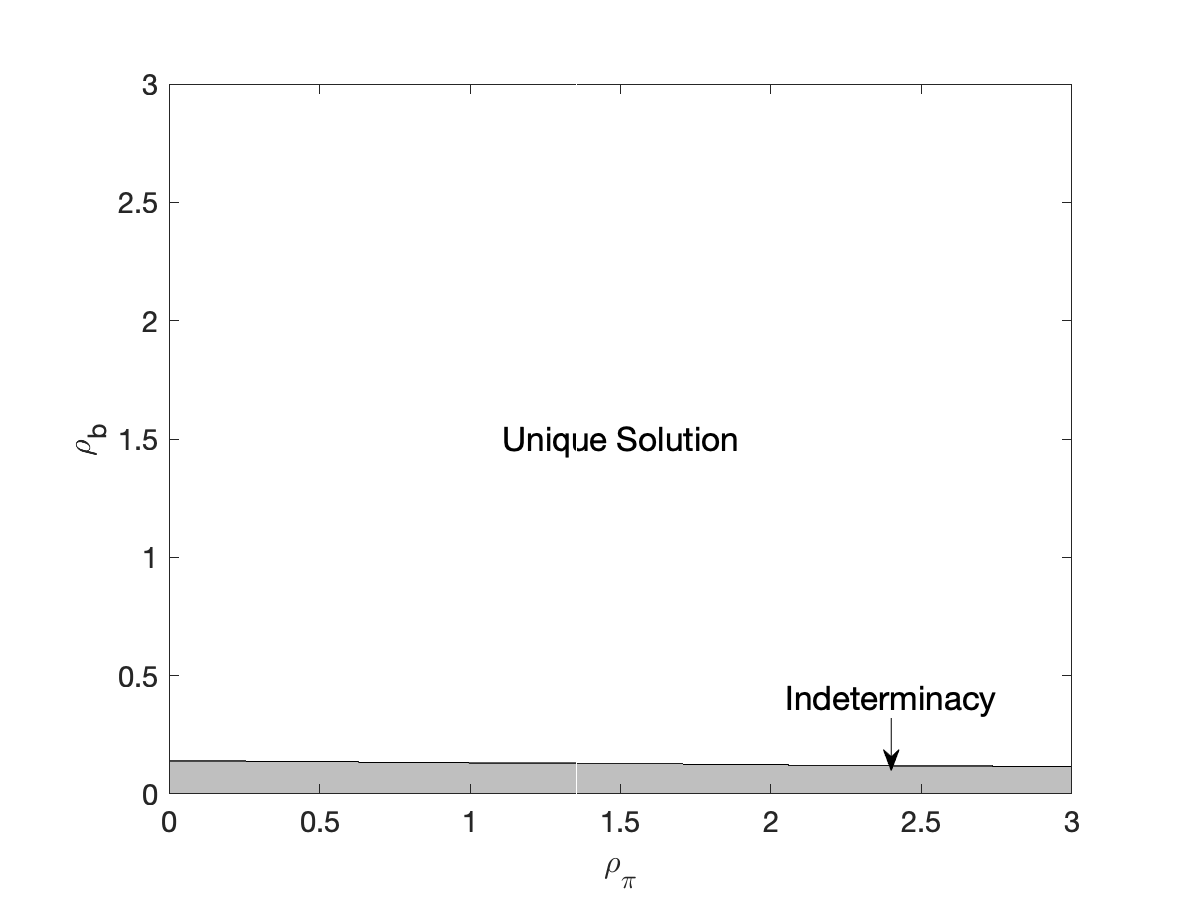
\includegraphics[width=0.85\textwidth]{FiscalMonetary_DeterminacyRegions_1.eps}
\end{figure} 
\begin{figure}[p]
\centering
\caption{Impulse Response Functions for Policy Shocks}
\vspace{0.3em}
\label{fig:IRF_Policy}
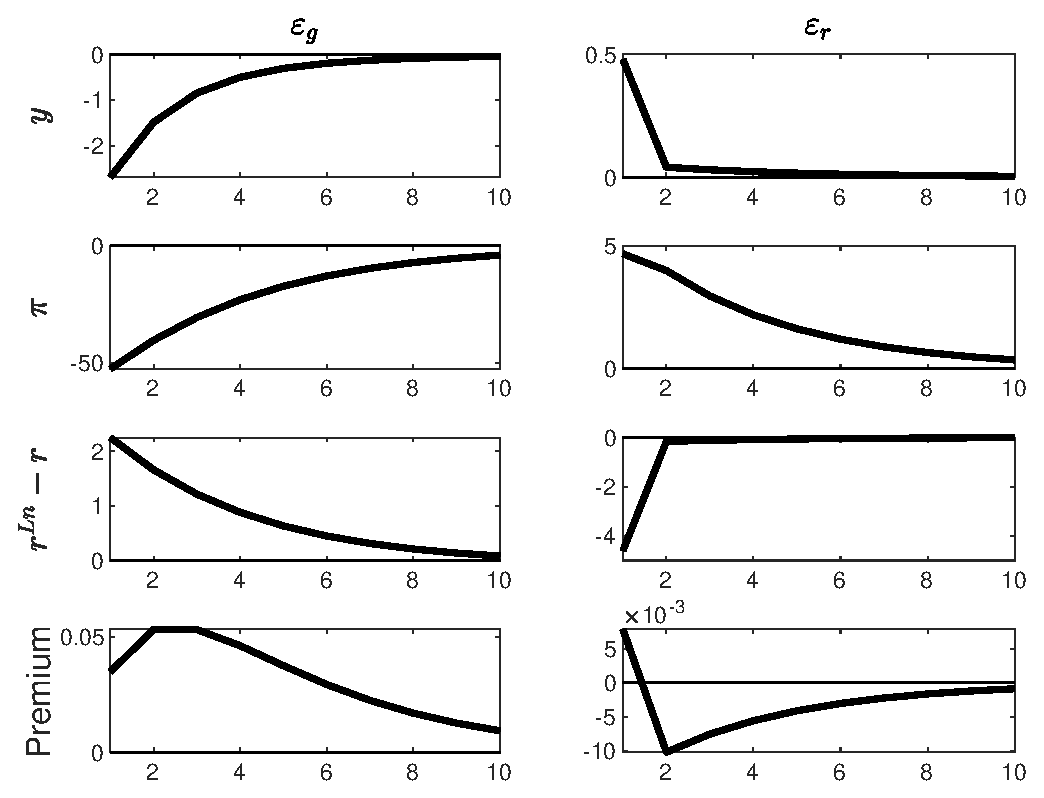
\includegraphics[width=0.75\textwidth]{IRF_Policy.eps}
\end{figure} 

The determination of the price level for nearly all parameterizations of the monetary policy rule stems from the combination of long-term debt existence and the imperfect substitutability within the utility function.
Consider the linearized first-order conditions that set the short- and long-term rates
\begin{equation}
\label{eq:ShortRates}
	\tilde{r}_t = \eta_1 \left[\mathbb{E}_t\tilde{c}_{t+1} - \tilde{c}_t + \mathbb{E}_t\tilde{\pi}_{t+1}\right] - \eta_2 \left[\tilde{\gamma}_{2,t} + \frac{1}{\sigma}\left(\tilde{\epsilon}^s_t + \tilde{m}_t - \tilde{b}_t\right)\right]
\end{equation}
and
\begin{equation}
\label{eq:LongRates}
	\tilde{r}^{L,n}_t = \eta_3 \left[\mathbb{E}_t\tilde{c}_{t+1} - \tilde{c}_t + \mathbb{E}_t\tilde{\pi}_{t+1}\right] + \eta_4 \mathbb{E}_t\tilde{r}^{L,n}_{t+1} - \eta_5 \tilde{r}^L_t - \eta_6 \left[\tilde{\gamma}_{2,t} + \frac{1}{\sigma}\left(\tilde{\epsilon}^s_t + \tilde{m}_t - \tilde{b}^L_t\right)\right],
\end{equation}
where $\{\eta_i\}_{i=1}^6$ are positive combinations of the model parameters. 
In both equations, the last bracketed terms are the premiums.\footnote{
	These could also be accounting for these assets' safety or collateral attributes.
	I use the term ``liquidity premium" for convenience.}
As will be explained below, these premiums are the channels through which fiscal policy flows and monetary policy erodes.
%This suggests, all else constant, that an increase in the stock of government debt will work through the liquidity premiums to put upward pressure on interest rates.
%% along with our assumed positive monetary response to the inflationary pressures causes by increased government spending. 
%Additionally, the debt-in-the-utility-function aspect of the model provides additional substitution way from consumption (and the inflationary pressures it causes). 
%That is, so long as fiscal policy responds strongly enough to its own debt levels, the liquidity premiums work as an added stabilizer, providing the unique solution desired.

\paragraph{The Passivity of Monetary Policy}
In the traditional sense, the stance of monetary policy depends on how aggressively it responds to inflation \citep{Leeper:1991}.
A strong response is considered ``active,'' while a more dovish response is considered ``passive."
As can be seen in the second column (third row) of Figure \ref{fig:IRF_Policy}, while monetary policy does control the short term rate $r_t$, it has virtually no impact on the long-term bond rate $r^{L,n}_t$.\footnote{Because of this, it also has little impact on the benchmark rate $R_t$, either.}
Because of the household's ability to substitute (imperfectly) across its portfolio of bonds, monetary policy is effectively absorbed in a way that makes it passive at all times. 
This can also be seen in the variance decomposition of the model, where the monetary policy shock accounts for less than one percent of the variations in the long-term bond rate. 

\paragraph{Fiscal Policy and Determinacy}
Equations (\ref{eq:ShortRates}) and (\ref{eq:LongRates}) show how fiscal policy, with a large enough tax response to new debt issuance, can simultaneously determine the price level and the debt level.
Due to their place in the utility function, rising debt levels cause a satiation effect, reducing the ``convenience'' of holding bonds and pushing both short- and long-term rates up.\footnote{
	The overall monetary services aggregate $m_t$ is also included in this liquidity premium, though the combination of the direct stock effect (via $b^{L,n}_t$ or $b_t$) and the assumed fall in the marginal utility of the monetary services $\gamma_{2,t}$ that would come from such an increase, are likely to overshadow this channel
	The adjustment in the monetary services aggregate is also relatively small due to its inclusion of fiat currency, providing a substitute in monetary services.}
This, coupled with the resulting movements in the marginal utilities of the consumption and monetary services bundles and rising taxes, create a more pronounced substitution away from consumption and the inflationary pressure it brings.
Thus, the fiscal authority only needs to account for the debt level. 

\paragraph{The Household and Determinacy}
With the fiscal authority effectively determining both the price and debt levels, determinacy of the equilibrium in this model boils down to how ``active'' the household is in establishing the distribution of its debt portfolio.
%Determinacy of the equilibrium in this model boils down to the fiscal authority's ability to manage the overall debt level and the strength of the household's preferences in identifying the distribution in the portfolio.
That is, the household has the have strong enough preferences across the various securities to stabilize the distribution of the portfolio.
Figure \ref{fig:Determinacy_RhoSigma} shows the determinacy regions in the $(\rho_b, \sigma)$ space, where again the shaded area denotes indeterminacy of the equilibrium.
\begin{figure}[h]
\centering
\caption{Determinacy Properties: Fiscal Policy and Portfolio Preferences}
\vspace{0.3em}
\label{fig:Determinacy_RhoSigma}
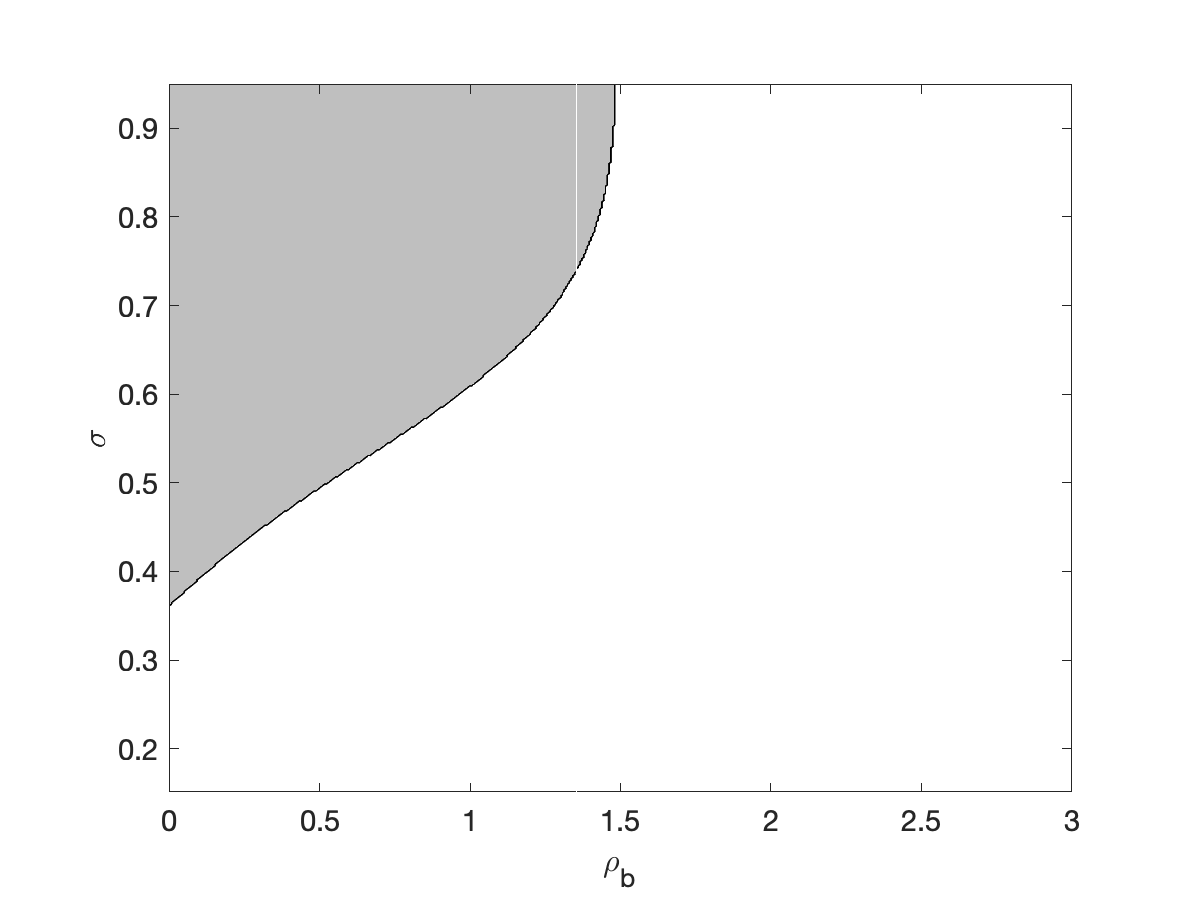
\includegraphics[width=0.75\textwidth]{FiscalMonetary_DeterminacyRegions_sigmab.eps}
\end{figure} 

%Considering the rest of the model, Figure \ref{fig:IRF_Policy} shows that, while the effects of monetary policy might suggest it, the model overall does not replicate the fiscal theory of the price level for the standard parameter space.
%In this instance, the existence of liquidity/safety properties means that increased government debt does not provide the wealth effect suggested by the FTPL. 
%What is new to this model is that, while the model is calibrated such that $\rho_b = 0.5$, the presence of long-term bonds eliminates the need for fiscal policy to be active \citep[in the][sense]{Leeper:1991} for this deflationary effect to hold.
%
%On the monetary-policy side, the impulse response functions also shed light on the rather small impact of monetary policy in determining the dynamics of the model. 
%The spread between the long- and short-term bonds ($r^{L,n}_t - r_t$) suggests that there is some leakage in this standard channel. 
%Short-term rates rise according to policy, but long-term rates are sluggish to do so. 
%This, combined with fiscal policy directly in the rate premiums, would imply that monetary policy may have less impact than our standard models suggest. 

In summary, the determinacy properties of the parameters space do not align with the traditional \citet{Leeper:1991} paradigm. 
The inclusion of debt in the utility function and the substitutability across types of debt therein effectively negate the impact of monetary policy in establishing a unique equilibrium. 
So while this suggests that fiscal policy is more impactful in determining the price level, this is not through the standard FTPL channel. 

Lastly, as can be seen in Figure \ref{fig:IRF_Policy}, the results of this small-scale model are a bit more extreme than the data would suggest. 
For instance, a government spending shock $\epsilon^g_t$ has a negative output multiplier due to an extreme crowding-out effect on consumption.
While a negative consumption multiplier is standard in these small-scale models, the magnitude seen here is new. 
Therefore, this model should be considered as motivation for potential channels of policy only.
A more extensive analysis of this class of model, however, is beyond the scope of this paper and is therefore left to future research.

\section{Fiscal Monetary Services and Inflation}
\label{sec:Empirical}
To what degree does fiscal policy, and its debt specifically, influence inflation rates and the price level?
While it has been difficult to find a link between the principal value of outstanding fiscal debt and inflation, in this section I consider the theoretical implications of the model above and again consider a \citet{Jorda:2005} linear projection model to empirically explore the impact of these fiscal monetary services on inflation.
Given the myriad of likely inflationary channels, estimating impulse response functions via local projections allows me more flexibility to incorporate more variables while simultaneously providing more protection against omitted variable bias.

\subsection{The Theoretical Model}
Equations (\ref{eq:ShortRates}) and (\ref{eq:LongRates}) not only shed light on the dynamic interactions between the monetary and fiscal authorities, but also provide insight on how the monetary services provided by government debt can lead to inflation via the liquidity premium.
The term $\epsilon^s_t$ represents a shock to the contribution of monetary services provided by government debt.
As the equations show, an increase in the monetary services can be inflationary due to downward pressure on interest rates. 
Figure (\ref{fig:IRF_Inflation_eps}) shows the response of inflation to a one-percent increase in the contribution of the overall debt portfolio to monetary services. 
\begin{figure}[h]
\centering
\caption{IRF: Inflation to a Government Debt Monetary Services Shock}
\label{fig:IRF_Inflation_eps}
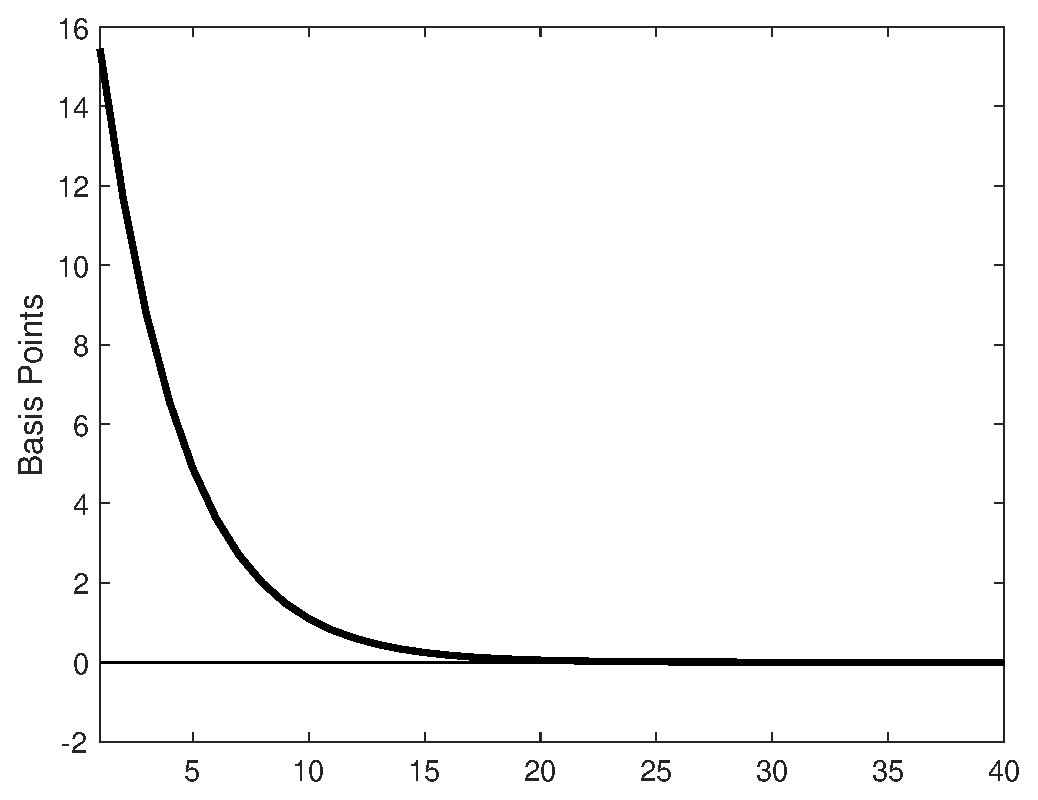
\includegraphics[width=0.85\textwidth]{IRF_Inflation_ep_s.eps}
\end{figure} 

It should be kept in mind that this model includes neither habit formation nor policy smoothing on either side.
Thus the impact from the model under the baseline calibration (see Appendix \ref{app:Model}), the response of inflation is immediate, but does provide the theoretical motivation for the inflationary pressures derived from fiscal monetary services.\footnote{While not shown here, this inflationary result is robust to variations in both the aggressiveness of policy and the elasticity of substitution in the debt portfolio across the entire determinant parameter space.}
The next step is to empirically test the impact of these fiscal monetary services on inflation.
%An empirical exploration of this can be found below.



\subsection{The Empirical Model}
\paragraph{Identification of Exogenous Shocks}
Exogenous shocks to the year-over-year growth rate of fiscal monetary services shown in Figure \ref{fig:YoY_growth} are derived using a model similar to (\ref{eq:Shock_ID}).
%$$
%	m_t = c + \Gamma(L)X_t + \epsilon_t,
%$$
%where $c$ is a constant term and 
Again, the control variables $X_t$ attempt to control for variations in the perceived monetary services resulting from general financial shocks and other external factors.
To control for the overall macroeconomic environment, I include the year-over-year changes in the Wilshire 5000 stock price index as well as the 10-year, 2-year yield curve spread.
Market expectations are controlled for using the index of consumer sentiment from the University of Michigan's Surveys of Consumers.
Default risk is proxied by the standard deviation of the daily Wilshire 5000 index similar to that of \citet{Krishnamurthy-VissingJorgensen:2012}.
Stock effects from increases/decreases in the amount of debt outstanding are controlled for using the growth rate of the simple sum aggregate.
Lastly, relative movements in the perceived services of other sovereign debt are controlled for using the trade-weighted US dollar index of major currencies.
All variables are nominal, where appropriate, and are monthly in frequency.
Four lags are considered based on AIC.
%These are chosen because much of the monetary services provided by these fiscal securities is determined by the economic environment and the expectations thereof. 
The residuals $\epsilon_t$ are the estimated exogenous shocks to the growth of fiscal monetary services.

\paragraph{Estimating the Impact on Inflation}
%The model considered here is linear
%$$
%	z_{t+h} = c_t + \Phi(L_h)y_t + \beta_h\epsilon_t + \varepsilon_{t+h},
%$$
%where $h$ is the forecast horizon, $z_{t+h}$ is the dependent variable, $\epsilon_t$ is the identified shock of choice, $y_t$ is the vector of control variables including lags of up to $L_h$, and $\beta_h$ form the estimated impulse response functions.
%The variable $c_t$ is a vector of trends includes the constant term as well as time trends ranging from linear to fourth-order.
Impulse response functions are estimated using a model with the same form as (\ref{eq:Jorda_Model}).
All the data in this analysis is monthly in frequency and---after adjustments for data availability and lag order in both the identification and estimation steps---covers the 1986:3--2019:12 period.
The dependent variable $z_{t+h}$ is the year-over-year growth rate of the personal consumption expenditures chain-type price index, excluding food and energy (core PCE inflation).
Given the potential for noise in month-over-month measures, using a year-over-year growth rate should provide a better perspective.
The control variables $y_t$ include lags of the unemployment rate, the 12-month ahead inflation expectations as measured by the University of Michigan's Surveys of Consumers, the nominal effective federal funds rate, the non-cyclical rate of unemployment, core PCE inflation, the year-over-year inflation rate of end-use import prices adjusted for their share of GDP, the year-over-year growth rate of nominal spot oil prices, and the growth rate of the simple-sum debt aggregate. 
Dummy variables indicating recessions and the zero lower bound are also included.
As is suggested by \citet{Kilian-Kim:2011}, the lag order is determined at each horizon, based on AIC, and with a maximum lag order of six.\footnote{
	It should be noted that this lag maximum is half that of the previous analyses.
	This is due to the AIC persistently suggesting that the model push against the maximum at nearly every horizon in this analysis.
	\citet{Kilian-Kim:2011} note that the models fit better when the maximum lag order is restricted, and allowing the maximum to be considerably higher does not fundamentally change the results.
	So to preserve sample size, a maximum lag order of six was chosen.}

%: Lag Structure
% Inflation - 3     2     6     6     6     6     6     6     6     6     6     6     6     6     5     4     4     3



%: IRF of Monetary Services Shock
\begin{figure}[h]
\centering
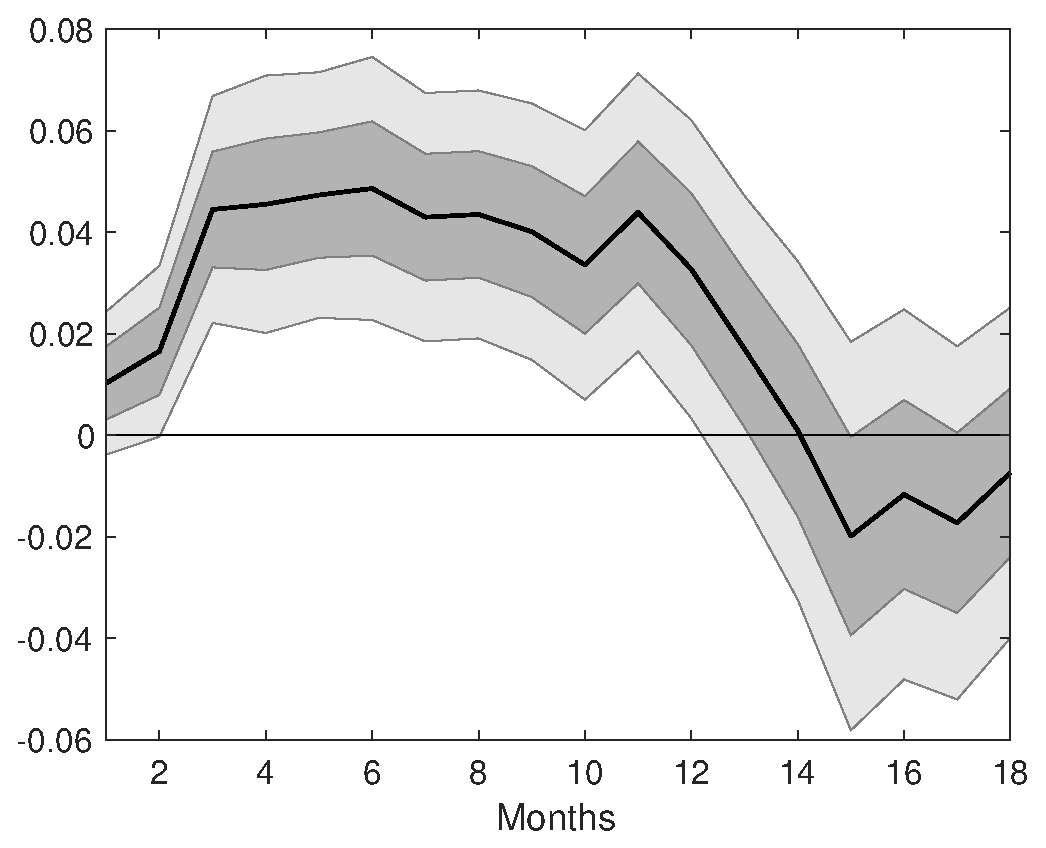
\includegraphics[width=0.85\textwidth]{Infl_SpreadShock.eps}
\caption{Inflationary Response to Fiscal Monetary Services Shock}
\label{fig:IRF}
\end{figure}
Figure \ref{fig:IRF} presents the impact of a one-percentage-point increase in fiscal monetary services on the core PCE inflation rate.
After a two-month lag, the year-over-year inflation rate peaks at 4.9 basis points and the statistical significance of the shock persists for about ten months.
%\footnote{
%	Despite the fact that positive and statistically-significance estimate can be seen after the 20-month point, I focus only on the first 24-months of estimates here so as to err on the conservative side.
%	The estimates are provided out to 36 months in the appendix.
%	There, the positive and statistically-significant results remain through the 30-month point.}
Given that the average year-over-year growth rate in the sample is approximately 2.5 percent and has frequently reached the 5-10 percent range, the impact of fiscal monetary services is both statistically significant and economically large. 


\paragraph{Implications for FTPL}
The results above have significant implications for the fiscal theory of the price level, though the direction of those implications depends on how one views the results.\footnote{
	I'd like to thank a number of conference participants who brought up this interesting debate.}
On the one hand, this is inflation driven by the issuance and usage of US marketable Treasury securities, which is evidence of a fiscal inflationary channel through government borrowing.
%This would be considered one of the first purely-empirical proofs of the theory, with much of the literature relying on estimation of large-scale New Keynesian models and their underlying assumptions.
On the other hand, some may still consider this as monetary in nature, proving Milton Friedman correct by providing solid evidence that even the inflation caused by fiscal policy is still monetary. 
Also, the model considered in Section \ref{sec:MonetaryFiscal} suggests that this result can arise without the need for the FTPL. 
More evidence will be needed to properly sort out this debate, including the use of larger-scale models that can explore the possible interaction/transition from this rate premium channel to the standard FTPL channel.


\section{Conclusion}
\label{sec:Conclusion}
The stock of outstanding US government debt has consistently increased since the early 2000s, yet interest rates and prices have only recently begun accelerating. 
Prior to that, borrowing costs continuously fell as government debt continuously rose.
This has prompted many to reconsider both the traditional views of government bonds and fiscal budgetary constraints \citep[e.g.][]{Krishnamurthy-VissingJorgensen:2012,Brunnermeier-Merkel-Sannikov:2022}.

In this paper, I use the idea that government securities provide monetary services to their holders to construct a Fisher ideal index of marketable US Treasury debt. 
I show that the value of these monetary services increases the fiscal capacity of the government---primarily through the safety they provide---in a simple partial equilibrium model with short- and long-term debt.
I then use this constructed metric, in comparison to the simple sum aggregate, to uncover the growth rate of these fiscally-provided monetary services and show that an increase has an inflationary impact that is persistently positive and both statistically and economically significant. 
These results suggest that there is a monetary services channel stemming from fiscal policy, but even small scale models can reproduce this without invoking the standard FTPL channels.
Overall, while finding evidence linking the stock of outstanding principal to the price level has been difficult to come by, my findings offer another plausible channel. 

\paragraph{Shortcomings and Future Research}
As no one has previously attempted an index-number approach to US Treasury debt, there are a number of opportunities for future research.
With regards to the measurement itself, removal of both Federal Reserve and foreign official holdings of debt may shed additional light on the monetary services provided by the Treasury.
Recent evidence suggest that this may not matter, however. 
\citet{Krishnamurthy-VissingJorgensen:2015}, in their analysis of Treasury debt's impact on financial market lending, also maintain SOMA holdings and find virtually no change in their results when foreign official holdings are removed from their metric of choice.
%So while this is a common concern when exploring Treasury debt, the evidence suggests that it may not matter.
Further research can test this hypothesis. 
Additionally, further development of the measurement should incorporate important concepts like uncertainty and risk aversion as well as testing for weak separability across the currently ad-hoc baskets of Treasury securities.
Assuming that these tests suggest fewer baskets than is currently in use, this would further help alleviate the issue of assets moving into and out of existence. 
As for the empirical analyses, a deeper look into the collateral services Treasury securities provide is warranted.
My initial approach to this can be found in Appendix \ref{app:MonetaryServices}, though the sample size and choice of the proxy variable leaves much to be desired.
As collateralized lending has continued to grow over recent decades, more data should become available to better assess this as a monetary service. 

Another avenue of future research that was alluded comes from the theory side.
In this paper, I explore the impact of liquidity and safety generally through the theoretical model and then attempt to separate them empirically. 
A larger-scale model would allow the separation of the liquidity and safety origins, potentially leading to a derivation that would allow the separation of them in the measurement itself. 
This possibility would then open the door to a number of additional tests of the impact of Treasury borrowing on financial markets and the economy, more generally.

\newpage

\bibliographystyle{apecon}
\bibliography{MonetaryServices_Debt}

\newpage
\appendix
\numberwithin{equation}{section}
\section{Representative Household Solution}
\label{app:HH_Solution}

Combining (\ref{eq:LoM_DebtLevel}) and (\ref{eq:LoM_DebtReturn})
\begin{equation}
	\left(r^L_t-r^{L,n}_t\right)B^L_t = (1-\alpha)\left(r^L_{t-1}-r^{L,n}_t\right)B^L_{t-1},
	\label{eq:CombEq_1}
\end{equation}
(\ref{eq:LoM_CapLevel}) and (\ref{eq:LoM_CapReturn})
\begin{equation}
	\left(R_t-R^{n}_t\right)K_t = (1-\delta)\left(R_{t-1}-R^{n}_t\right)K_{t-1},
	\label{eq:CombEq_2}
\end{equation}
and (\ref{eq:HH_Budget}), (\ref{eq:LoM_DebtLevel}), and (\ref{eq:LoM_CapLevel})
\begin{multline}
	B_t + B^{L}_t - (1-\alpha)B^L_{t-1} + p_tc_t + K_t - (1-\delta)K_{t-1} = (\delta^* + R_{t-1})K_{t-1} \\+ (1+r_{t-1})B_{t-1} + (\alpha + r^L_{t-1})B^L_{t-1} + (1-\tau_t)W_tl_t + \int^1_0\Pi_t(s)\text{d}s.
	\label{eq:CombEq_3}
\end{multline}

\subsection{Household's Problem}
(\ref{eq:HH_Utility}) subject to (\ref{eq:HH_MonServices}), (\ref{eq:CombEq_1}), (\ref{eq:CombEq_2}), and (\ref{eq:CombEq_3}). Choosing 
$\left\{B_t, B^L_t, c_t, K_t, R_t, r^L_t, l_t, M_t\right\}$

\subsection{Bellman Equation}

\begin{multline}
	\mathbb{V}\!\left(B_{t-1}, B^L_{t-1}, K_{t-1}, R_{t-1}, r^L_{t-1}\right) \\= \max \Bigg\{u(c_t) + v\left(\frac{M_t}{P_t}\right) + x(l_t)  + \beta\mathbb{E}_t\!\left[\mathbb{V}\!\left(B_{t}, B^L_{t}, K_{t}, R_{t}, r^L_{t}\right)\right] \\
	+ \frac{\mu_{1,t}}{p_t} \Big[(\delta^* + R_{t-1})K_{t-1} + (1+r_{t-1})B_{t-1} + (\alpha + r^L_{t-1})B^L_{t-1} + (1-\tau_t)W_tl_t \\+ \int^1_0\Pi_t(s)\text{d}s -B_t - B^{L}_t + (1-\alpha)B^L_{t-1} - p_tc_t - K_t + (1-\delta)K_{t-1}\Big] \\
	+ \frac{\mu_{2,t}}{p_t}\Bigg[\left[\lambda^{\frac{1}{\sigma}}B_t^{\frac{\sigma-1}{\sigma}} + (1-\lambda)^{\frac{1}{\sigma}}{B^L_t}^{\frac{\sigma-1}{\sigma}}\right]^{\frac{\sigma}{1-\sigma}}-M_t\Bigg] \\
	+ \frac{\mu_{3,t}}{p_t}\Big[(1-\delta)\left(R_{t-1}-R^{n}_t\right)K_{t-1} - \left(R_t-R^{n}_t\right)K_t \Big] \\
	+ \frac{\mu_{4,t}}{p_t} \Big[(1-\alpha)\left(r^L_{t-1}-r^{L,n}_t\right)B^L_{t-1} - \left(r^L_t-r^{L,n}_t\right)B^L_t\Big]\Bigg\}
	\label{eq:Bellman}
\end{multline}

\subsection{First Order Conditions}

\begin{equation}
	u'(c_t) = \mu_{1,t}
	\label{eq:HH_FOC_c}
\end{equation}
%
\begin{equation}
	v'\left(\frac{M_t}{p_t}\right) = \mu_{2,t}
	\label{eq:HH_FOC_M}
\end{equation}
%
\begin{equation}
	x'(l_t) + \mu_{1,t} \frac{W_t}{p_t} (1-\tau_t) = 0
	\label{eq:HH_FOC_l}
\end{equation}
%
\begin{equation}
	\beta\mathbb{E}_t\!\left[\mathbb{V}\!_1\left(B_{t}, B^L_{t}, K_{t}, R_{t}, r^L_{t}\right)\right] = \frac{\mu_{1,t}}{p_t} - \frac{\mu_{2,t}}{p_t}\left(\frac{\lambda M_t}{B_t}\right)^{\frac{1}{\sigma}}
	\label{eq:HH_FOC_B}
\end{equation}
%
\begin{equation}
	\beta\mathbb{E}_t\!\left[\mathbb{V}\!_2\left(B_{t}, B^L_{t}, K_{t}, R_{t}, r^L_{t}\right)\right] = \frac{\mu_{1,t}}{p_t} - \frac{\mu_{2,t}}{p_t}\left(\frac{(1-\lambda) M_t}{B^L_t}\right)^{\frac{1}{\sigma}} + \frac{\mu_{4,t}}{p_t}\left(r^L_t - r^{L,n}_t\right)
	\label{eq:HH_FOC_BL}
\end{equation}
%
\begin{equation}
	\beta\mathbb{E}_t\!\left[\mathbb{V}\!_3\left(B_{t}, B^L_{t}, K_{t}, R_{t}, r^L_{t}\right)\right] = \frac{\mu_{1,t}}{p_t} + \frac{\mu_{3,t}}{p_t}\left(R_t - R^{n}_t\right)
	\label{eq:HH_FOC_K}
\end{equation}
%
\begin{equation}
	\beta\mathbb{E}_t\!\left[\mathbb{V}\!_4\left(B_{t}, B^L_{t}, K_{t}, R_{t}, r^L_{t}\right)\right] = \frac{\mu_{3,t}}{p_t}K_t
	\label{eq:HH_FOC_R}
\end{equation}
%
\begin{equation}
	\beta\mathbb{E}_t\!\left[\mathbb{V}\!_5\left(B_{t}, B^L_{t}, K_{t}, R_{t}, r^L_{t}\right)\right] = \frac{\mu_{4,t}}{p_t}B^L_t
	\label{eq:HH_FOC_rL}
\end{equation}

\subsection{Bienveniste-Scheinkman Conditions}

\begin{equation}
	\mathbb{V}\!_1\left(B_{t-1}, B^L_{t-1}, K_{t-1}, R_{t-1}, r^L_{t-1}\right) = \frac{\mu_{1,t}}{p_t}(1+r_{t-1})
	\label{eq:HH_BS_B}
\end{equation}
%
\begin{equation}
	\mathbb{V}\!_2\left(B_{t-1}, B^L_{t-1}, K_{t-1}, R_{t-1}, r^L_{t-1}\right) = \frac{\mu_{1,t}}{p_t}(1+r^L_{t-1}) + \frac{\mu_{4,t}}{p_t}(1-\alpha)\left(r^L_{t-1} - r^{L,n}_t\right)
	\label{eq:HH_BS_BL}
\end{equation}
%
\begin{equation}
	\mathbb{V}\!_3\left(B_{t-1}, B^L_{t-1}, K_{t-1}, R_{t-1}, r^L_{t-1}\right) = \frac{\mu_{1,t}}{p_t}(\delta^*- \delta + 1 + R_{t-1}) + \frac{\mu_{3,t}}{p_t}(1-\delta)\left(R_{t-1} - R^{n}_t\right)
	\label{eq:HH_BS_K}
\end{equation}
%
\begin{equation}
	\mathbb{V}\!_4\left(B_{t-1}, B^L_{t-1}, K_{t-1}, R_{t-1}, r^L_{t-1}\right) = \left(\frac{\mu_{1,t}}{p_t} + (1-\delta)\frac{\mu_{3,t}}{p_t}\right)K_{t-1}
	\label{eq:HH_BS_R}
\end{equation}
%
\begin{equation}
	\mathbb{V}\!_5\left(B_{t-1}, B^L_{t-1}, K_{t-1}, R_{t-1}, r^L_{t-1}\right) = \left(\frac{\mu_{1,t}}{p_t} + (1-\alpha)\frac{\mu_{4,t}}{p_t}\right)B^L_{t-1}
	\label{eq:HH_BS_rL}
\end{equation}

\subsection{Optimality Conditions}

\begin{equation}
	u'(c_t) = \mu_{1,t}
	\label{eq:HH_OC_c}
\end{equation}
%
\begin{equation}
	v'\left(\frac{M_t}{p_t}\right) = \mu_{2,t}
	\label{eq:HH_OC_M}
\end{equation}
%
\begin{equation}
	x'(l_t) + \mu_{1,t} \frac{W_t}{p_t} (1-\tau_t) = 0
	\label{eq:HH_OC_l}
\end{equation}
%
\begin{equation}
	\frac{\mu_{1,t}}{p_t} - \frac{\mu_{2,t}}{p_t}\left(\frac{\lambda M_t}{B_t}\right)^{\frac{1}{\sigma}} = \beta\mathbb{E}_t\!\left[\frac{\mu_{1,t+1}}{p_{t+1}}(1+r_t)\right]
	\label{eq:HH_OC_B}
\end{equation}
%
\begin{multline}
	\frac{\mu_{1,t}}{p_t} - \frac{\mu_{2,t}}{p_t}\left(\frac{(1-\lambda) M_t}{B^L_t}\right)^{\frac{1}{\sigma}} + \frac{\mu_{4,t}}{p_t}\left(r^L_t - r^{L,n}_t\right) \\ = \beta\mathbb{E}_t\!\left[\frac{\mu_{1,t+1}}{p_{t+1}}(1+r^L_{t}) + \frac{\mu_{4,{t+1}}}{p_{t+1}}(1-\alpha)\left(r^L_{t} - r^{L,n}_{t+1}\right)\right] 
	\label{eq:HH_OC_BL}
\end{multline}
%
\begin{multline}
	\frac{\mu_{1,t}}{p_t} + \frac{\mu_{3,t}}{p_t}\left(R_t - R^{n}_t\right) \\ = \beta\mathbb{E}_t\!\left[\frac{\mu_{1,t+1}}{p_{t+1}}(\delta^*- \delta + 1 + R_{t}) + \frac{\mu_{3,{t+1}}}{p_{t+1}}(1-\delta)\left(R_{t} - R^{n}_{t+1}\right)\right]
	\label{eq:HH_OC_K}
\end{multline}
%
\begin{equation}
	\frac{\mu_{3,t}}{p_t}K_t = \beta\mathbb{E}_t\!\left[\frac{\mu_{1,t+1}}{p_{t+1}} + (1-\delta)\frac{\mu_{3,{t+1}}}{p_{t+1}}\right]K_t
	\label{eq:HH_OC_R}
\end{equation}
%
\begin{equation}
	\frac{\mu_{4,t}}{p_t}B^L_t = \beta\mathbb{E}_t\!\left[\frac{\mu_{1,t+1}}{p_{t+1}} + (1-\alpha)\frac{\mu_{4,{t+1}}}{p_{t+1}}\right]B^L_t
	\label{eq:HH_OC_rL}
\end{equation}

\newpage
\section{Derivation of the User Costs}
\label{app:usercost_derivation}

Combining (\ref{eq:HH_manOC_K}) and (\ref{eq:HH_manOC_R}) yields:
\begin{equation}
	1 = \beta\mathbb{E}_t \Bigg[ \frac{\mu_{t+1}}{\mu_{t}}\frac{1}{\pi_{t+1}} \Big\{ 1 + R^n_t + \delta^* - \delta - (1-\delta)\gamma_{3,t+1}\Delta R^n_{t+1}\Big\}\Bigg]
	\label{eq:HH_manOC_K+R}
\end{equation}
%\begin{multline}
%	1 - \beta\mathbb{E}_t\left[\frac{\mu_{1,t+1}}{\mu_{1,t}} \frac{1}{\pi_{t+1}}\right]R^n_t = \beta\mathbb{E}_t\left[\frac{\mu_{1,t+1}}{\mu_{1,t}} \frac{1}{\pi_{t+1}}\right](\delta^*-\delta) \\ 
%	+ \beta\mathbb{E}_t\left[\frac{\mu_{1,t+1}}{\mu_{1,t}} \frac{1}{\pi_{t+1}}\right] - \beta\mathbb{E}_t\left[\frac{\mu_{1,t+1}}{\mu_{1,t}} \frac{1}{\pi_{t+1}}(1-\delta)\gamma_{3,t+1}\Delta R^n_{t+1}\right]
%\end{multline}
Substituting this for the 1 in (\ref{eq:HH_manOC_B}) and rearranging yields the marginal benefit/marginal cost equilibrium:
\begin{equation}
	\gamma_{2,t}\left(\frac{\lambda M_t}{B_t}\right)^\frac{1}{\sigma} = \beta\mathbb{E}_t \Bigg[ \frac{\mu_{t+1}}{\mu_{t}}\frac{1}{\pi_{t+1}} \Big\{ R^n_t + \delta^* - \delta - (1-\delta)\gamma_{3,t+1}\Delta R^n_{t+1} - r_t \Big\}\Bigg]
\end{equation}
%\begin{multline}
%	\gamma_{2,t}\left(\frac{\lambda M_t}{B_t}\right)^\frac{1}{\sigma} = \beta\mathbb{E}_t\left[\frac{\mu_{1,t+1}}{\mu_{1,t}} \frac{1}{\pi_{t+1}}\right](R^n_t - r_t) \\ 
%	- \beta\mathbb{E}_t\left[\frac{\mu_{1,t+1}}{\mu_{1,t}} \frac{1}{\pi_{t+1}}(1-\delta) \gamma_{3,t+1}\Delta R^n_{t+1}\right] + \beta\mathbb{E}_t\left[\frac{\mu_{1,t+1}}{\mu_{1,t}} \frac{1}{\pi_{t+1}}\right](\delta^*-\delta)
%\end{multline}
Now dividing both sides by (\ref{eq:HH_manOC_K+R}) converts the right side to the standard user cost form
\begin{equation}
	\gamma_{2,t}\left(\frac{\lambda M_t}{B_t}\right)^\frac{1}{\sigma} = \frac{\mathbb{E}_t \Big[ \frac{\mu_{t+1}}{\mu_{t}}\frac{1}{\pi_{t+1}} \Big\{ R^n_t + \delta^* - \delta - (1-\delta)\gamma_{3,t+1}\Delta R^n_{t+1} - r_t \Big\}\Big]}{\mathbb{E}_t \Big[ \frac{\mu_{t+1}}{\mu_{t}}\frac{1}{\pi_{t+1}} \Big\{ 1+ R^n_t + \delta^* - \delta - (1-\delta)\gamma_{3,t+1}\Delta R^n_{t+1}\Big\}\Big]}
	\label{eq:HH_manOC_usercost}
\end{equation}
Decoupling $\gamma_{2,t}$ shows that the right hand side is the marginal cost of holding the short-term asset, expressed in terms of utility.
\begin{equation}
	v'\!\!\left(\frac{M_t}{p_t}\right)\!\!\left(\frac{\lambda M_t}{B_t}\right)^\frac{1}{\sigma} = u'(c_t)\frac{\mathbb{E}_t \Big[ \frac{\mu_{t+1}}{\mu_{t}}\frac{1}{\pi_{t+1}} \Big\{ R^n_t + \delta^* - \delta - (1-\delta)\gamma_{3,t+1}\Delta R^n_{t+1} - r_t \Big\}\Big]}{\mathbb{E}_t \Big[ \frac{\mu_{t+1}}{\mu_{t}}\frac{1}{\pi_{t+1}} \Big\{ 1+ R^n_t + \delta^* - \delta - (1-\delta)\gamma_{3,t+1}\Delta R^n_{t+1}\Big\}\Big]}
\end{equation}
%Now incorporating (\ref{eq:HH_OC_c}) and (\ref{eq:HH_OC_M}):
%\begin{multline}
%	v'\!\left(\frac{M_t}{p_t}\right)\left(\frac{\lambda M_t}{B_t}\right)^\frac{1}{\sigma} = u'(c_t)\Bigg\{\beta\mathbb{E}_t\left[\frac{\mu_{1,t+1}}{\mu_{1,t}} \frac{1}{\pi_{t+1}}\right](R^n_t - r_t) \\ 
%	- \beta\mathbb{E}_t\left[\frac{\mu_{1,t+1}}{\mu_{1,t}} \frac{1}{\pi_{t+1}}(1-\delta) \gamma_{3,t+1}\Delta R^n_{t+1}\right] + \beta\mathbb{E}_t\left[\frac{\mu_{1,t+1}}{\mu_{1,t}} \frac{1}{\pi_{t+1}}\right](\delta^*-\delta)\Bigg\}
%\end{multline}

If it is assumed that that $\frac{\mu_{1,t+1}}{\mu_{1,t}} \frac{1}{\pi_{t+1}}$ is independent of the one-period returns in brackets, this expression simplifies even further to 
\begin{equation}
	\eta_t = \frac{R^n_t + \delta^* - \delta - (1-\delta)\mathbb{E}_t[\gamma_{3,t+1}\Delta R^n_{t+1}] - r_t }{ 1+ R^n_t + \delta^* - \delta - (1-\delta)\mathbb{E}_t[\gamma_{3,t+1}\Delta R^n_{t+1}]},
	\label{eq:usercost_ST}
\end{equation}
where $\eta_t$ equals the left-hand side of (\ref{eq:HH_manOC_usercost}) and represents the user cost of holding the short term asset for one period.
%\begin{equation}
%v'\!\left(\frac{M_t}{p_t}\right)\left(\frac{\lambda M_t}{B_t}\right)^\frac{1}{\sigma} = u'(c_t)\Bigg\{\frac{R^n_t - (1-\delta)\mathbb{E}_t\left[\gamma_{3,t+1}\Delta R^n_{t+1}\right] + (\delta^*-\delta) - r_t}{1+ R^n_t - (1-\delta)\mathbb{E}_t\left[\gamma_{3,t+1}\Delta R^n_{t+1}\right] + (\delta^*-\delta)}\Bigg\},
%\label{eq:usercost_ST}
%\end{equation}

Beginning the same procedure from (\ref{eq:HH_manOC_BL}) will provide the analogous user cost for a long-term security
\begin{equation}
\eta^L_t = \frac{\mathbb{E}_t \Big[ \frac{\mu_{t+1}}{\mu_{t}}\frac{1}{\pi_{t+1}} \Big\{ R^n_t + \delta^* - \delta - (1-\delta)\gamma_{3,t+1}\Delta R^n_{t+1} - r^{L,n}_t + (1-\alpha)\gamma_{4,t+1}\Delta r^{L,n}_{t+1}\Big\}\Big]}{\mathbb{E}_t \Big[ \frac{\mu_{t+1}}{\mu_{t}}\frac{1}{\pi_{t+1}} \Big\{ 1+ R^n_t + \delta^* - \delta - (1-\delta)\gamma_{3,t+1}\Delta R^n_{t+1}\Big\}\Big]},
%\label{eq:usercost_LT}
\end{equation}
and again assuming independence as above yields
\begin{equation}
\eta^L_t = \frac{R^n_t + \delta^* - \delta - (1-\delta)\mathbb{E}_t[\gamma_{3,t+1}\Delta R^n_{t+1}] - r^{L,n}_t + (1-\alpha)\mathbb{E}_t[\gamma_{4,t+1}\Delta r^{L,n}_{t+1}]}{1+ R^n_t + \delta^* - \delta - (1-\delta)\mathbb{E}_t[\gamma_{3,t+1}\Delta R^n_{t+1}]}.
\label{eq:usercost_LT}
\end{equation}
Since we're dealing with long-term assets here, the period-by-period user cost incorporates both the expected one-period payouts as well as the expected capital gains/loses.
The capital gains are incorporated via the expected change in the one-period payouts, scaled by the expected future price of the asset.

\newpage
\section{The Full Model}
\label{app:Model}

The contributions of the model are primarily derived from the household's problem.
Here, however, I outline the remainder of the model for further analysis.

\subsection{The Representative Household}
The initial setup allowed the various utility functions to remain flexible.
Here I assign a logarithmic functional form to consumption $u(c_t) = \ln{c_t}$ and constant relative risk aversion (CRRA) functions to real monetary services $v(m_t) = \frac{m_t^{1-\nu} -1}{1-\nu}$ and leisure hours $x(1-l_t) = \chi \frac{(1-l_t)^{1+\psi}-1}{1+\psi}$. 

\subsection{Final Goods-Producing Firm}
A final goods-producing firm acts as a retailer, aggregating the intermediate goods $i\in[0,1]$ into a consumable bundle with production CES production function
\begin{equation}
\label{eq:FinalGoods_Production}
	y_t = \left[\int^1_0 y_t(i)^{\frac{\theta-1}{\theta}}\mathrm{d}i\right]^\frac{\theta}{\theta-1}.
\end{equation}
This firm operates in a perfectly competitive market, choosing the quantity of each intermediate good $y_t(i)\; \forall i$ that maximizes profits
\begin{equation}
\label{eq:FinalGoods_Profit}
	\Pi_t^f = p_ty_t - \int_0^1p_t(i)y_t(i)\mathrm{d}i.
\end{equation}
Doing so leads to the standard demand function for the intermediate goods
\begin{equation}
\label{eq:FinalGoods_FOC}
	y_t(i) = \left(\frac{p_t(i)}{p_t}\right)^{-\frac{1}{\theta}}y_t \; \forall i.
\end{equation}

\subsection{Intermediate Goods Producing Firms}
The intermediate goods-producing firms operate in a monopolistically-competitive environment, hiring labor $l_t(i)$ and utilizing a linear production technology $y_t(i) = z_tl_t(i)$, where $z_t$ is a common technology that follows the stationary auto-regressive process
\begin{equation}
\label{eq:Technology}
	\ln z_t = (1-\rho_z)\ln z + \rho_z \ln z_{t-1} + \varepsilon^z_t,
\end{equation}
where $\rho_z \in (0,1)$ and $\varepsilon^z_t \sim \mathcal{N}(0,\sigma^2_z)$.
In maximizing their profits, the intermediate firms face a Rotemburg quadratic cost of price adjustment $\phi\left(\frac{p_t(i)}{\pi_t p_{t-1}(i)} - 1\right)^2y_t$, measured in term of the final output.
Choosing the price of its respective intermediate good to maximize profits subject to the demand of the final-goods firm and assuming a symmetric equilibrium yields the a linearized Phillips curve relationship
\begin{equation}
\label{eq:NKPC}
	\tilde{\pi}_t = \beta\mathbb{E}_t\tilde{\pi}_{t+1} + \frac{\theta}{\phi}(\tilde{w}_t - \tilde{z}_t),
\end{equation}
where the tilde denotes the variable's percent deviation from its steady state value.

\subsection{Fiscal and Monetary Policy}

The government's budget constraint is straight-forward in that the fiscal authority takes in revenue via a lump sum tax $\tau_t$ and borrowing at both short $B_t$ and long $B^{L,n}_t$ maturities. 
Real spending $g_t$ is considered to be exogenous
\begin{equation}
\label{eq:GovSpending}
	\ln g_t = (1-\rho_g)\ln g + \rho_g\ln g_{t-1} + \varepsilon^g_t,
\end{equation}
where $\rho_g \in (0,1)$, $g$ is the steady state value of real government spending, and $\varepsilon^g_t \sim \mathcal{N}(0,\sigma_g^2)$. 
Together with the law of motion for long-term debt (\ref{eq:LoM_DebtLevel}), the real fiscal budget constraint is
\begin{equation}
\label{eq:FiscalBudget}
	g_t + \frac{F_t}{p_t} + (1+r_{t-1})\frac{B_{t-1}}{p_t} + (1+r^L_{t-1})\frac{B^L_{t-1}}{p_t} = \tau_t + \frac{F_{t-1}}{p_t}+\frac{B_t}{p_t} + \frac{B^L_t}{p_t}
\end{equation}

\subsection{Equilibrium Conditions and Calibration}

In equilibrium, $k_t = 0$ and $f_t = f$ for all $t$ and $\pi_t = \frac{p_t}{p_{t-1}}$ is the gross inflation rate.

Calibration of this model starts with a standardized steady state aggregate output $y = 1$ and debt-GDP ratio of one-hundred percent ($b + b^L = y$). 
The steady state value of currency is derived from the ratio of total public federal debt to the monetary base, which is 8.13 during the 1982--2022 period, suggesting $f = 0.12$.
The weight on currency in the monetary aggregate $\lambda_1 = 0.74$ is calculated from the relative user costs on the monetary assets. 
The average 10-year treasury constant maturity rate during this same period is about 5.73 percent, which is considered as the steady state value of $r^L_t$. 
The weights on short-term and long-term debt are calibrated such that a 1.25 percentage point spread exists between the short-term and long-term rates, which is roughly in line with the average 10yr--3m yield curve spread during the 1982--2022 period. 
This yields values of $\lambda_2 = 0.1089$ and $\lambda_3 = 0.1511$. 
The parameter governing the elasticity of substitution $\sigma$, is set at 0.40. 
\citet{Belongia-Ireland:2014} uses 0.50 for the elasticity across currency and deposits. 
Assuming currency and deposits are closer to perfect substitutes than long- and short-term debt this would be the upper bound on the analogous parameter in this model.
The assumption of 10-year bonds above implies $\alpha = \delta = 0.025$.

The discount factor $\beta = 0.9624$ matches a two percent inflation target $\pi = 1.02$ and the spread on the benchmark rate $R - r^L = 0.0025$ as assumed in the derivation of the monetary aggregate in Section \ref{sec:DataMethodology}.
I also follow \citet{Belongia-Ireland:2014} in setting $\theta = 6$ and $\phi=50$, which imply a 20 percent markup over the intermediate goods and full price adjustment over a period of 3.75 quarters.
For the baseline analysis, I assume no smoothing to the policy rates $\rho_\tau = \rho_r = 0$, and policy values of $\rho_\pi = 1.5,\, \rho_y = 0$, and $\rho_b = 0.5$ to ensure determinacy when evaluating impulse responses.


\newpage
\section{Derivation of the Government's Budget Constraint}
\label{app:govt_budget}

Starting with a standard government budget constraint (abstracting from currency for this part) with short- and long-term bonds, and given (\ref{eq:usercost_ST}) and (\ref{eq:usercost_LT}) and some rearranging, we can simplify the above equation to
%\begin{multline}
%	\frac{B_{t-1}+B^L_{t-1}}{p_t}(1+r_{t-1}) = t_t - g_t - (r^L_{t-1}-r_{t-1})\frac{B^L_{t-1}}{p_t} \\
%		+ \beta\mathbb{E}\left[\frac{\mu_{1,t+1}}{\mu_{1,t}}\frac{B_t+B^L_t}{p_{t+1}}(1+r_{t})\right] + \eta_t\frac{B_t+B^L_t}{p_{t}},
%\end{multline}
\begin{multline}
	\frac{B_{t-1}(1+r_{t-1})+B^L_{t-1}(1+r^L_{t-1})}{p_t} = t_t - g_t \\ + \beta\mathbb{E}_t\left[\frac{\mu_{1,t+1}}{\mu_{1,t}} \frac{B_{t}(1+r_{t})+B^L_{t}(1+r^L_{t})}{p_{t+1}}\right] +  \eta_t\frac{B_t}{p_t} +\eta^L_t\frac{B^L_t}{p_t}\\
		+ \left\{ \beta \mathbb{E}_t\left[ \frac{\mu_{t+1}}{\mu_t}\frac{1}{\pi_{t+1}} \left(r^{L,n} - (1-\alpha)\gamma_{4,t+1}\Delta r^{L,n}_{t+1}\right)\right] - \beta \mathbb{E}_t\left[\frac{\mu_{t+1}}{\mu_t}\frac{1}{\pi_{t+1}}\right]r^L_t\right\} \frac{B^L_t}{p_t}
%		+ (1-\alpha)\beta\mathbb{E}_t\left[\frac{\mu_{1,t+1}}{\mu_{1,t}} \frac{B^L_t \gamma_{4,t+1}\left(r^L_t - r^{L,n}_{t+1}\right)}{p_{t+1}}\right] - \gamma_{4,t}\left(r^L_t - r^{L,n}_t\right)\frac{B^L_t}{p_t}
\end{multline}
where $\eta_t$ and $\eta^L_t$ are the user costs of short-term and long-term debt as described in (\ref{eq:usercost_ST}) and (\ref{eq:usercost_LT}), respectively.
Next, I use (\ref{eq:HH_manOC_K+R}) to add zero into the term in brackets and then divide the left section of that term by one 
 \begin{multline}
	\frac{B_{t-1}(1+r_{t-1})+B^L_{t-1}(1+r^L_{t-1})}{p_t} = t_t - g_t \\ 
		+ \beta\mathbb{E}_t\left[\frac{\mu_{1,t+1}}{\mu_{1,t}} \frac{B_{t}(1+r_{t})+B^L_{t}(1+r^L_{t})}{p_{t+1}}\right] +  \eta_t\frac{B_t}{p_t} +\eta^L_t\frac{B^L_t}{p_t}\\
		+ \Bigg\{-\frac{\mathbb{E}_t \Big[ \frac{\mu_{t+1}}{\mu_{t}}\frac{1}{\pi_{t+1}} \Big\{ R^n_t + \delta^* - \delta - (1-\delta)\gamma_{3,t+1}\Delta R^n_{t+1} - r^{L,n}_t + (1-\alpha)\gamma_{4,t+1}\Delta r^{L,n}_{t+1}\Big\}\Big]}{\mathbb{E}_t \Big[ \frac{\mu_{t+1}}{\mu_{t}}\frac{1}{\pi_{t+1}} \Big\{ 1+ R^n_t + \delta^* - \delta - (1-\delta)\gamma_{3,t+1}\Delta R^n_{t+1}\Big\}\Big]} \\
		- \beta \mathbb{E}_t\left[\frac{\mu_{t+1}}{\mu_t}\frac{1}{\pi_{t+1}}\right](1+ r^L_t)\Bigg\} \frac{B^L_t}{p_t}.
\end{multline}

\newpage
\section{Monetary Services of Treasury Bills versus Notes/Bonds}
\label{app:MonetaryServices}

In this section, I re-construct the processes described in Sections \ref{sec:DataMethodology} and \ref{subsec:MonetaryServices} using cross sections of the data that isolate the nominal bills from the nominal notes and bonds. 
This includes the recalculation of the benchmark rates used in each statistical index number.

\subsection{Impact on Safety}
The impact of an increase in the monetary services of Treasury bills on the Baa--Aaa corporate bond spread can be seen in Figure \ref{fig:Safety_Bills}.
As can be seen, the estimate is positive for a persistent amount of time, with statistically significance of the impact coming in the fifth and sixth months after the shock.
This impact is temporary, however, and suggests a reduction in market safety at later horizons. 
Overall, these results suggest that Treasury bills do provide safety to the market. 
%: IRF of Monetary Services Shock on Safety-Bills
\begin{figure}[p]
\centering
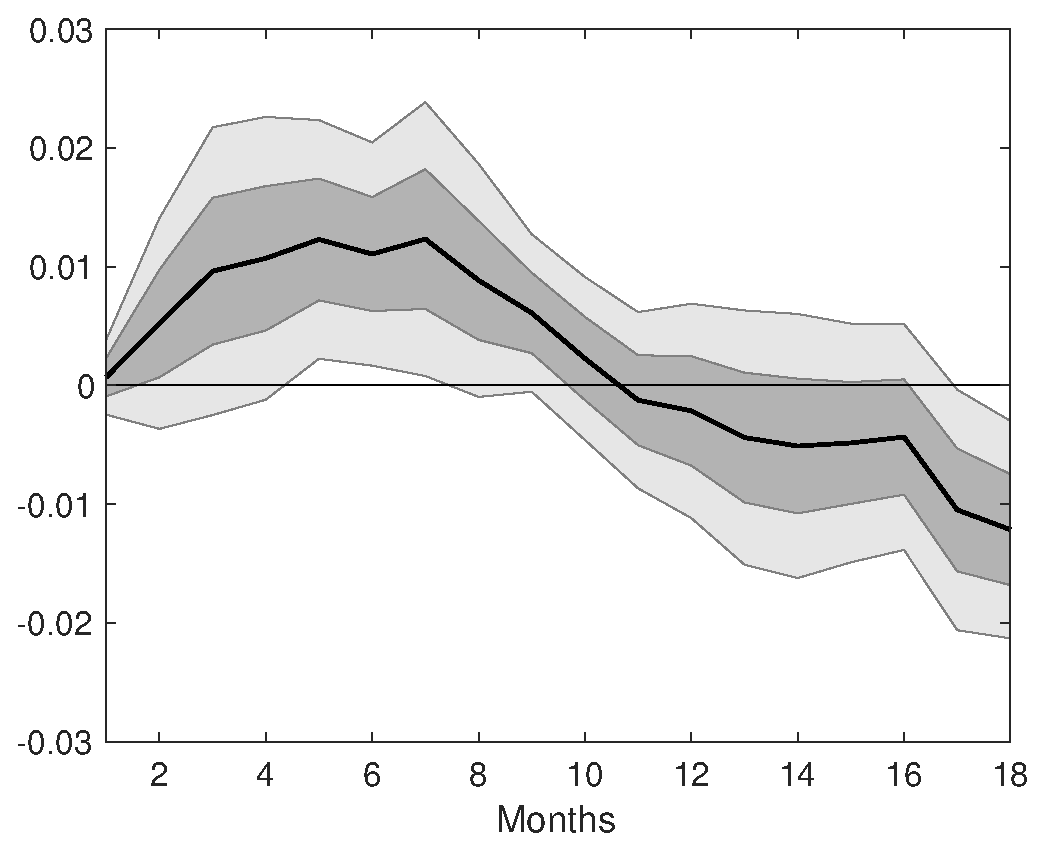
\includegraphics[width=0.7\textwidth]{Attributes_Bills_Safety.eps}
\caption{Impact of Monetary Services on Baa--Aaa Spread: Treasury Bills}
\label{fig:Safety_Bills}
\end{figure}

The impact of an increase in this measure of the monetary services of Treasury notes and bonds on the same spread can be seen in Figure \ref{fig:Safety_Bonds}.
The larger estimates, coupled with greater persistence, suggests that the reduction in the price of safety seen in the full portfolio (Figure \ref{fig:Attributes_Safety}) is largely driven by the combination of notes and bonds.
Both this result and that of the Treasury bills reaffirms the narrative that US Treasuries are a primary source of market safety.  
%: IRF of Monetary Services Shock on Safety-Bonds
\begin{figure}[p]
\centering
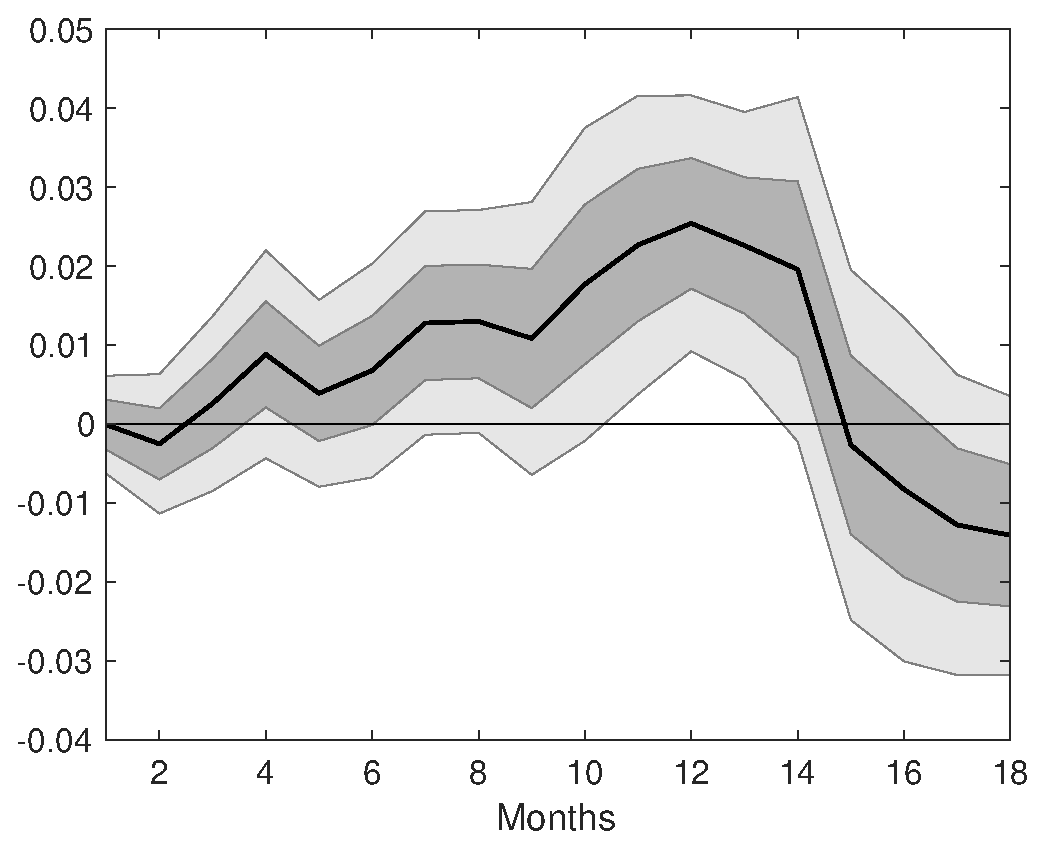
\includegraphics[width=0.7\textwidth]{Attributes_Bonds_Safety.eps}
\caption{Impact of Monetary Services on Baa--Aaa Spread: Treasury Notes/Bonds}
\label{fig:Safety_Bonds}
\end{figure}

\subsection{Impact on Liquidity}
The impact of an increase in the monetary services of Treasury bills on the Aaa--10yr spread can be found in Figure \ref{fig:Liquidity_Bills}.
Treasury bills are shown to have no statistical impact on market liquidity in the first eight months.
Thereafter, it seems that bills reduce market liquidity (increase the price of liquidity) in the market 10-months later. 
This suggests that bills are just as liquid in the very short run as the currency/reserves that are being extracted by their issuance, resulting in a net-zero impact at best.
%: IRF of Monetary Services Shock on Liquidity-Bills
\begin{figure}[p]
\centering
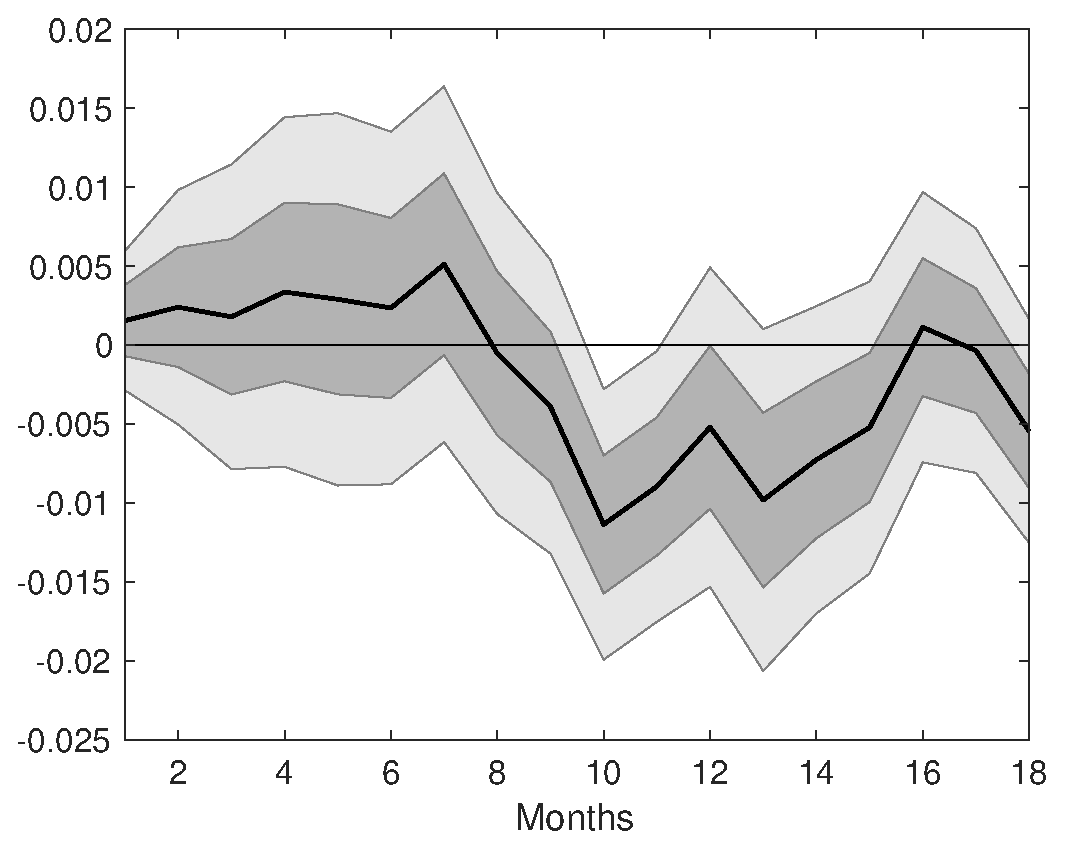
\includegraphics[width=0.7\textwidth]{Attributes_Bills_Liquidity.eps}
\caption{Impact of Monetary Services on Aaa--10yr Spread: Treasury Bills}
\label{fig:Liquidity_Bills}
\end{figure}

Treasury notes and bonds, however, reduce the liquidity in the market on impact, as can be seen in Figure \ref{fig:Safety_Bonds}.
This estimate, which is only statistically significant for the first and last two-month windows of the horizon, remains negative for the full duration of the estimate.
These results combined add to findings of \citet{Amihud-Mendelson:1991} and the simple analysis conducted in Section \ref{subsec:MktSeg}, that bills are dramatically more liquid that notes and bonds. 
So much so that notes and bonds reduce liquidity in the market.
%: IRF of Monetary Services Shock on Liquidity-Bills
\begin{figure}[p]
\centering
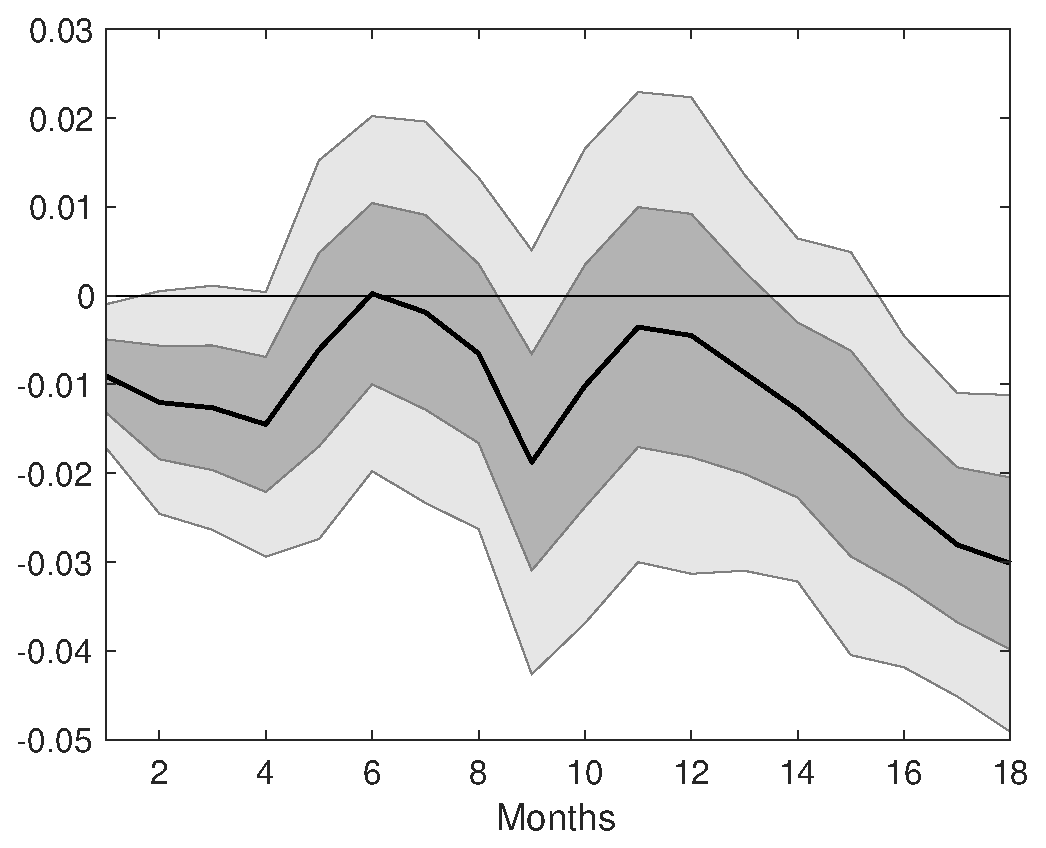
\includegraphics[width=0.7\textwidth]{Attributes_Bonds_Liquidity.eps}
\caption{Impact of Monetary Services on Aaa--10yr Spread: Treasury Notes/Bonds}
\label{fig:Liquidity_Bonds}
\end{figure}

\subsection{Impact on Collateral}
To assess the impact of the Treasury's portfolio on collateral values, consider an increase in the fiscally-provided monetary services on the spread between the 90-day AA non-financial commercial paper and 90-day AA asset-backed commercial paper interest rates, which acts a proxy for the value of collateral in the market.
That is, do these monetary services also include its use as collateral?
A decrease in this spread signals an increase in demand for secured lending, suggesting that the securities are seen as more useful/valuable as collateral.

It should be noted that the interest rates of concern only date back to January 2001, making the sample size much smaller than the other exercises.
So while the same model is considered, the maximum number of lags is set at three to compensate for the lack of observations.
I also remove the Aaa--10yr spread from the control variables, though the results are robust to variations in this choice. 

The results can be seen in Figures \ref{fig:Collateral_Bills} and \ref{fig:Collateral_Bonds}.
The unsecured--secured lending spread initially falls with an increase in the monetary services of bills, suggesting that an increase in these securities creates more demand for repo-style, secured borrowing.
Thus, the monetary services of bills includes their use as collateral.
On the other hand, we see a small but opposite initial effect of an increase in the monetary services of notes/bonds, suggesting that they do not 
Therefore, combined with the results in Figures \ref{fig:Safety_Bonds} and \ref{fig:Liquidity_Bonds}, the monetary services of notes/bonds is exclusively safety. 
%: IRF of Monetary Services Shock on Collateral-Bills
\begin{figure}[p]
\centering
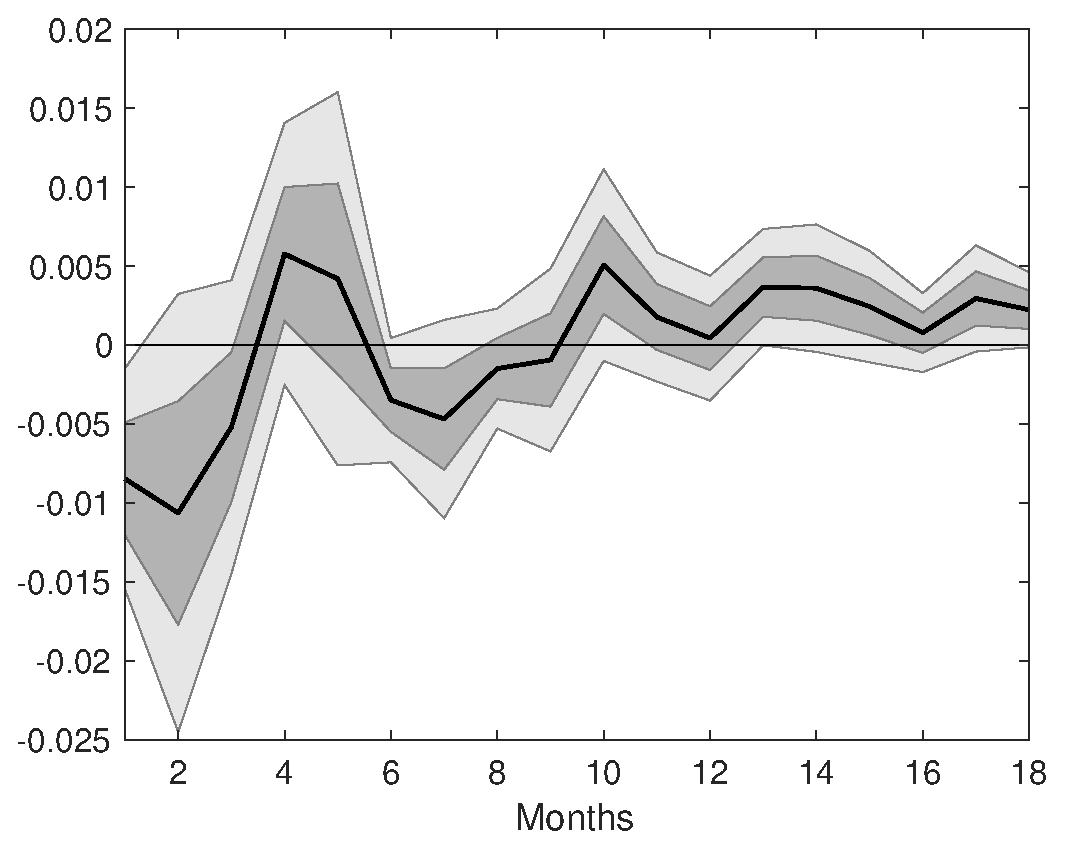
\includegraphics[width=0.7\textwidth]{Attributes_Bills_Collateral.eps}
\caption{Impact of Monetary Services on Unsecured vs Secured Lending Rates: Treasury Bills}
\label{fig:Collateral_Bills}
\end{figure}

%: IRF of Monetary Services Shock on Collateral-Bills
\begin{figure}[p]
\centering
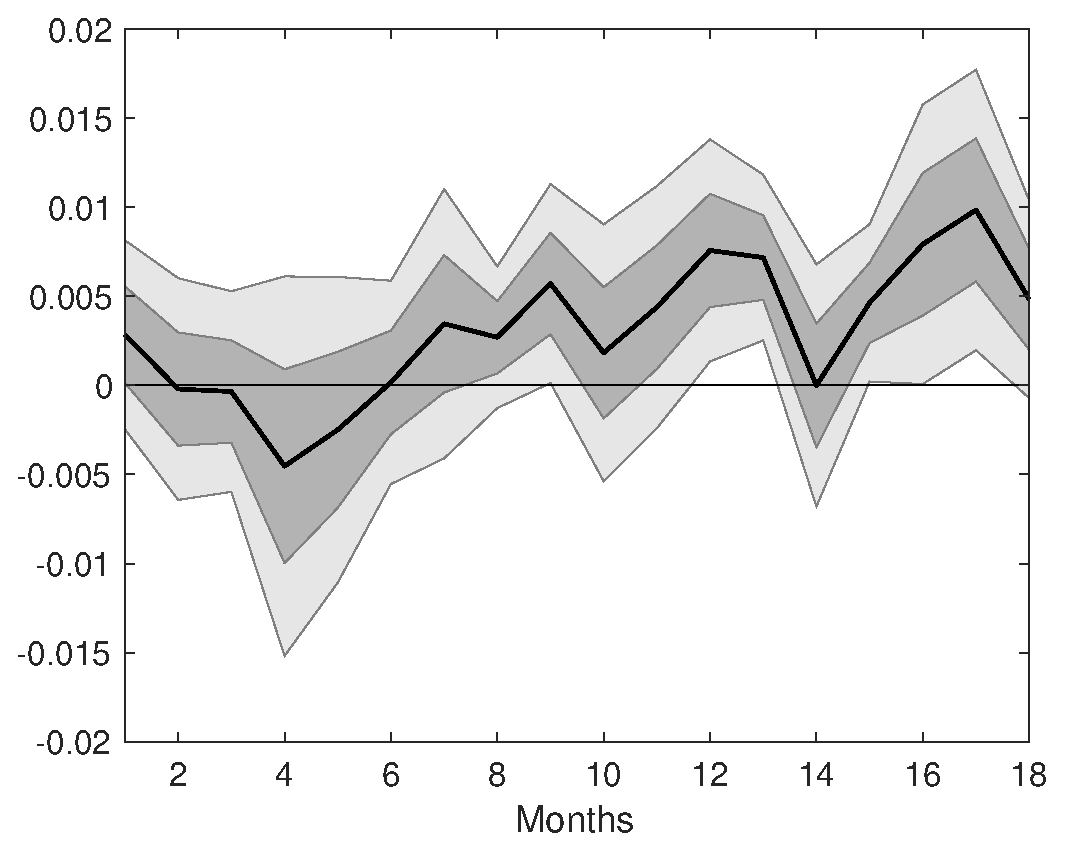
\includegraphics[width=0.7\textwidth]{Attributes_Bonds_Collateral.eps}
\caption{Impact of Monetary Services on Unsecured vs Secured Lending Rates: Treasury Notes/Bonds}
\label{fig:Collateral_Bonds}
\end{figure}

\end{document}